% paper_e.tex  
%    A manuscript sample for submission to Transactions of the Institute of 
%    Systems, Control and Information Engineers

%Authors: Please do not make any changes on the commands below.
%%%%%%%%%%%%%%%%%%%%%%%%%%%%%%%%%%%%%%%%%%%%%%%%%%%%%%%%%%%%%%%%%%%%%%%%%%%%%%
\documentclass[E]{scitrans}
%\usepackage{graphicx}
\usepackage{math}
\usepackage{bm}
\usepackage[dvipdfmx]{graphicx,xcolor}
\usepackage[dvipdfmx]{epsfig}
%
\appearyear{0000}
\vol{0}
\numberinvol{0}
\setcounter{page}{1}
\setcounter{volumepage}{1}
\Transaction
%%\Shortpaper
\ForSubmission
%Authors: Please do not make any changes on the commands above.
%%%%%%%%%%%%%%%%%%%%%%%%%%%%%%%%%%%%%%%%%%%%%%%%%%%%%%%%%%%%%%%%%%%%%%%%%%%%%%


%%Authors: If you wish to use packages, please include them here.
%%         Note that only "amsfonts" and "psfrag" packages are available.
%%         The "latexsym" package has been already included.
%\usepackage{amsfonts}
%\usepackage{psfrag}

%Authors: Please follow the format below to fill in: paper's title, authors' 
%         names and affiliations, paper's condensed title and authors' names,
%         abstract and keywords.
%%%%%%%%%%%%%%%%%%%%%%%%%%%%%%%%%%%%%%%%%%%%%%%%%%%%%%%%%%%%%%%%%%%%%%%%%%%%%%
\begin{document}

\title{DESIGN OF A TWO-PIECE BRASSIERE CUP TO FIT BREAST DATA POINTS TOWARD ITS AUTOMATION}

\author{Kotaro {\sc Yoshida}${}^\dagger$, Hidefumi {\sc Wakamatsu}${}^\dagger$, Eiji {\sc Morinaga}${}^\ddagger$, and Takahiro {\sc Kubo}${}^\S$}

%Authors: Please write paper's short title and authors' names.
\headingtitle{DESIGN BRASSIERE CUP TO FIT BREAST DATA POINTS}
\headingauthors{{\sc Yoshida}, {\sc Wakamatsu}, {\sc Morinaga} and {\sc Kubo}}

%Authors: Please copy the abstract of your paper.
\abstract{
       A method to design the two-dimensional shapes of patterns of two piece brassiere cup is proposed when its target three-dimensional shape is given as a cloud of its data points. A brassiere cup consists of several patterns and their shapes are designed by repeatedly making a paper cup model and checking its three-dimensional shape. For improvement of design efficiency of brassieres, such trial and error must be reduced. As a cup model for check is made of paper not cloth, it is assumed that the surface of the model is composed of several developable surfaces. When two lines lying on a developable surface are given, the shape of the surface can be determined. Then, the two-piece brassiere cup can be designed by minimizing the error between the surface and given data points. It was mathematically verified that the original developable surface can be reproduced from data points on it by use of our proposed method.
}

%Authors: Please do not make any changes on the commands below.
%%%%%%%%%%%%%%%%%%%%%%%%%%%%%%%%%%%%%%%%%%%%%%%%%%%%%%%%%%%%%%%%%%%%%%%%%%%%%%
\maketitle
\acceptdate{August 1, 1995}
\address{*}{\AcceptDate}
%Authors: Please do not make any changes on the commands above.

%%% In accordance with the ISCIE policy on overlapping conference/journal submissions, if the material of this paper originates from conference papers published in the proceedings of conferences or symposia organized by the ISCIE as preliminary report, the following line should be written at the footnote in the first page of this paper.
\address{*}{The material of this paper was partially presented at the International Symposium on Flexible Automation 2020 which was held in July, 2020.}

%%%%%%%%%%%%%%%%%%%%%%%%%%%%%%%%%%%%%%%%%%%%%%%%%%%%%%%%%%%%%%%%%%%%%%%%%%%%%%

%Authors: Please write down authors' affiliations and addresses.
\address{**}{Graduate School of Engineering,
	Osaka University;
	Yamadaoka, Suita city, Osaka 565-0871, JAPAN}
\address{***}{Graduate School of Humanities and Sustainable System Sciences,Osaka Prefecture University, 1-1, Gakuencho, Naka-ku, Sakai, Osaka 599-8531, Japan}
\address{****}{Wacoal Holdings Corporation;
	Nakajima-cho, Kisshoin, Minami-ku,Kyoto 601-8530, JAPAN}

%Authors: Please write down the keywords of your paper.
\keywords{design, simulation, theory of surfaces, automation}

%Authors: Please remove \input and write down the body of your paper.
%\section{Introduction}
This document describes how to use the \LaTeX2e class file, named 
``{\tt scitrans.cls}'', for Transactions of the Institute of Systems, 
Control and Information Engineers (ISCIE). 

{\tt scitrans.cls} works together with the following nine files: 
\begin{itemize}
\item {\tt scitrans.cls}
\item {\tt sci209.sty, scij.sty, scie.sty, scims.sty}
\item {\tt JT1scimc.fd, JT1scigt.fd}
\item {\tt JY1scimc.fd, JY1scigt.fd}
\end{itemize}
Please make sure that all these files are placed in the same directory 
as the source file and should not be modified.


\section{Sections, etc.}
This is an example of \verb+\section{ }+.

\subsection{Subsections}
This is an example of \verb+\subsection{ }+.

\subsubsection{Sub-Subsections}
This is an example of \verb+\subsubsection{ }+.


\paragraph{Paragraphs}
This is an example of \verb+\paragraph{ }+.
Please insert a blank line before \verb+\paragraph{ }+.


\subparagraph{Subparagraphs}
This is an example of \verb+\subparagraph{ }+.
Please insert a blank line before \verb+\subparagraph{ }+.


\section{Theorems, etc.}
In the {\tt scitrans.cls} class file,
theorems and related structures such as definition, lemma, proposition,
corollary, example, assumption, remark and proof are handled. 
For example,

\begin{theorem}
\label{theorem:1}
This is an example of the theorem environment.
The usage of the lemma, definition, proposition, corollary,
example and assumption environments 
are the same as that of the theorem environment.
\end{theorem}

\begin{proof}
This is an example of the proof environment. 
At the end of each proof, asterisks ``**'' are automatically placed
as the Q.E.D.\ symbol,
whereas they will be replaced by the symbol ``$\Box$'' in the final manuscript.
\end{proof}

\begin{remark}
\label{remark:1}
This is an example of the remark environment. 
\end{remark}

If the author wishes to declare a new theorem-like environment, 
\verb+newtheoremenv+ and \verb+newparenenv+ can be used.
For example,

\begin{newtheoremenv}{Question}
This is an example of declaring a new environment by \verb+newtheoremenv+.
\end{newtheoremenv}
\begin{newparenenv}{Answer}
This is an example of declaring a new environment by \verb+newparenenv+.
\end{newparenenv}



\section{Equations}
Equations are created by the traditional {\tt equation} environment. 
In order to produce multiline equations,
the {\tt eqnarray} environment can be used.
For example, 

\begin{eqnarray}
        \dot{\mbf{x}}(t) & = & A \mbf{x}(t) + B \mbf{u}(t) 
                               + \sum_{k=1}^N \Gamma_k \mbf{d}k(t)
                \label{eq:1}\\
        \mbf{y}(t) & = & C \mbf{x}(t) + D \mbf{u}(t)
                \label{eq:2}\\
        \mbf{u}(t) & = & F \mbf{x}(t)
                \label{eq:3}
\end{eqnarray}

\begin{subequations}  \label{eq:4}  
  \begin{eqnarray}
    \lefteqn{ 
        \frac{1}{2\pi} \int_{-\infty}^\infty 
        {\rm Tr}\, \{ \mbf{G}\T(-j\omega) \mbf{G}(j\omega) \} \, d\omega 
     }    \hspace*{2\zw} \nonumber \\
    & = & 
    \frac{1}{2\pi} \int_{-\infty}^\infty 
    {\rm Tr}\, \{  B\T (-j\omega I -A\T)^{-1}C\T \nonumber \\
    &   & 
    \times C (j\omega I - A)^{-1}B \}\, d\omega 
               \label{eq:4a} \\
    & = & 
    \frac{1}{2\pi j}\int_{-j\infty}^{j\infty} 
    {\rm Tr}\, \left\{ 
    \left[ \begin{array}{c|c} 
       A & B \\ \hline 
       C & 0 \end{array} \right]^\sim  
    \left[ \begin{array}{c|c} 
       A & B \\ \hline 
       C & 0 \end{array} \right]
    \right\} \, ds  
              \label{eq:4b} 
\end{eqnarray}
\end{subequations}

In multiline equations,
please pay attention to the message ``\verb+Overfull \hbox+'', 
and the equations should be composed with the proper length.

With the \verb+subequations+ environment, sub-equation numbers such as 
\Req{eq:4a}, \Req{eq:4b} can be achieved.
In equations, bold fonts can be output by using \verb+\mbf+ command.
The superscript ${\rm T}$ which expresses the transpose of a matrix and $\hinf$ 
can be achieved by \verb+\T+ and \verb+\hinf+ respectively.

For in-line equations, please use $\displaystyle \sum_{k=1}^N$
instead of $\sum_{k=1}^N$.
Similarly, the rule is applicable to \verb+\lim+, \verb+\max+, \verb+\min+,
etc.
For super and subscripts,
please use $X_a^b$ (\verb+$X_a^b$+) instead of ${X_a}^b$ (\verb+${X_a}^b$+).


\section{Figures and Tables}
%----------------------------
\begin{figure}[b]
        \centering
	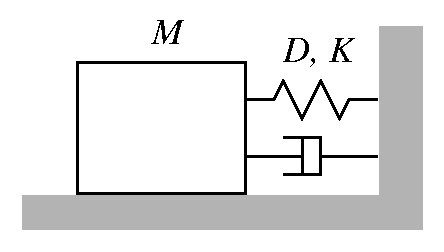
\includegraphics[width=5cm,clip]{tmp.eps}
        \caption{Mass-spring-damper system}
        \label{fig:1}
\end{figure}
%----------------------------
%
%----------------------------
\setlength{\unitlength}{10mm}
%

\begin{figure}[b]
        \centering
%
        \begin{picture}(4.5,1)(0,0)
                \thicklines
                \put(0,0.5){\vector(1,0){1.5}}
                \linethickness{1.2pt}
                \put(1.5,0){\framebox(1.5,1){$G(s)$}}
                \thicklines
                \put(3,0.5){\vector(1,0){1.5}}
        \end{picture}
%
        \caption{Plant}
        \label{fig:2}
\end{figure}
%----------------------------
%
%----------------------------
\begin{figure}[b]
        \centering
%
        \begin{picture}(5.5,2.5)(0,0)
                \thicklines
                \put(0,2){\vector(1,0){0.85}}
                \put(0.7,2.2){\makebox(0,0){$ \scriptstyle + $}}
                \put(1,2){\circle{0.3}}
                \thicklines
                \put(1.15,2){\vector(1,0){0.85}}
                \linethickness{1.2pt}
                \put(2,1.5){\framebox(1.5,1){$G(s)$}}
                \thicklines
                \put(3.5,2){\line(1,0){1}}
                \put(4.5,2){\circle*{0.08}}
                \put(4.5,2){\vector(1,0){1}}
                \put(4.5,2){\line(0,-1){1.5}}
                \put(4.5,0.5){\vector(-1,0){1}}
                \linethickness{1.2pt}
                \put(2,0){\framebox(1.5,1){$H(s)$}}
                \thicklines
                \put(2,0.5){\line(-1,0){1}}
                \put(1,0.5){\vector(0,1){1.35}}
                \put(0.8,1.7){\makebox(0,0){$ \scriptstyle - $}}
        \end{picture}
%
        \caption{Feedback control system}
        \label{fig:3}
\end{figure}

Graphics files (EPS files) can be inserted into a manuscript by 
\verb+\includegraphics+ command of the {\tt graphicx} package
(see \rfig{fig:1}). 
Here are some examples to insert graphics into a manuscript.
The {\tt picture} environment is also available
to draw figures (see \rfig{fig:2,fig:3}).

%
\begin{table}[h]
  \centering
  \caption{Example of table ({\tt slashbox.sty})}
  \label{table:1}
        \vspace{0.5\baselineskip}
  \begin{tabular}{!l!*{2}{c|}c!}\hlinethick
  \backslashbox{Room}{Date}
    &\makebox[3em]{5/31} &\makebox[3em]{6/1} &\makebox[3em]{6/2}\\ \hlinethick
    Room A	& --- & --- & --- \\ \hline
    Room C12	& --- & --- & --- \\ \hline
    Room F1201	& --- & --- & --- \\ \hlinethick
  \end{tabular}
\end{table}
%

Here is an example of a table. 
In the {\tt scitrans.cls},
the \verb+\tabular+ command has been extended for the ISCIE format.
The \verb+\tabular+ command provides the thin and thick lines.
The thin line can be achieved by the traditional way: ``\verb+|+''
for the vertical line and ``\verb+\hline+'' for the horizontal line.
The thick line can be achieved by ``\verb+!+'' and ``\verb+\hlinethick+''
for the vertical and horizontal thick lines respectively.

The {\tt arydshln.sty} is included in the {\tt scitrans.cls}
so that dashed lines are also available. 
Examples are shown in \rtab{table:2,table:3}.

%----------------------------
\begin{table}[hbt]
        \centering
        \caption{Commands for reference}
        \label{table:2}

        \vspace{0.5\baselineskip}

        \hdashlinewidth=8pt
        \hdashlinegap=4pt
        \begin{tabular}{!c|l!} \hlinethick
                Definition  & \verb+\rdefinition+ \\ \hdashline
                Theorem     & \verb+\rtheorem+ \\ \hdashline
                Lemma       & \verb+\rlemma+ \\ \hdashline
                Proposition & \verb+\rproposition+ \\ \hdashline
                Corollary   & \verb+\rcorollary+ \\ \hdashline
                Example     & \verb+\rexample+ \\ \hlinethick
        \end{tabular}
\end{table}
%----------------------------
%
%
%----------------------------
\begin{table}[hbt]
        \centering
        \caption{Commands for reference to equations, figures and tables}
        \label{table:3}

        \vspace{0.5\baselineskip}

        \hdashlinewidth=2pt
        \hdashlinegap=2pt
        \begin{tabular}{!l|l!} \hlinethick
                Equation                 & \verb+\req+ \\ \hdashline
                Equation in appendices   & \verb+\Req+ \\ \hdashline
                Equation with sub-number & \verb+\Req+ \\ \hdashline
                Figure                   & \verb+\rfig+ \\ \hdashline
                Table                    & \verb+\rtab+ \\ \hlinethick
        \end{tabular}
\end{table}
%----------------------------


\section{Citations}
Citations can be made with the \verb+\cite+ command\cite{foo1}. 
The \verb+\cite*+ command automatically places a word ``Ref.''
before the reference number as ``\cite*{foo1}''.

The multiple citation such as
\verb+\cite{foo1,foo2}+ and \verb+\cite{foo2,foo3,foo4}+ 
achieves \mbox{}\cite{foo1,foo2} and \mbox{}\cite{foo2,foo3,foo4} respectively.


\section{Cross-Referencing}
In order to reference the definition, theorem etc.,
please use the commands listed in \rtab{table:2},
for example: \verb+\rtheorem{theorem:1}+, \verb+\rremark{remarl:1}+.

\rtheorem{theorem:1} is an example of the \verb+\rtheorem+ command.

\rremark{remark:1} is an example of the \verb+\rremark+ command.

For referencing the equation,
figure and table, please use the commands listed in \rtab{table:3}.
These commands automatically add appropriate words before reference numbers.
For example, 
%the commands \verb+\req{eq:1}+, \verb+\rfig{fig:1}+ and \verb+\rtab{table:1}+
achieve 

\begin{itemize}
  \item \verb+\req{eq:1}+ $\quad\Longrightarrow\quad$ \req{eq:1}
  \item \verb+\rfig{fig:1}+ $\quad\Longrightarrow\quad$ \rfig{fig:1}
  \item \verb+\rtab{table:1}+ $\quad\Longrightarrow\quad$ \rtab{table:1}
\end{itemize}
The multiple referencing can be also achieved, for example,
\begin{itemize}
  \item \verb+\req{eq:1,eq:2,eq:3}+ $\quad\Longrightarrow\quad$
	\req{eq:1,eq:2,eq:3}
  \item \verb+\rfig{fig:1,fig:2}+ $\quad\Longrightarrow\quad$ \rfig{fig:1,fig:2}
  \item \verb+\rtab{table:1,table:2}+ $\quad\Longrightarrow\quad$
	\rtab{table:1,table:2}
\end{itemize}
In order to use the same format through the manuscript,
please do not use traditional 
\verb+\ref+ command.


\section{Others}
\subsection{Footnote}
The footnote is available with \verb+\footnote+ command%
\footnote{This is an example of the {\tt \textbackslash footnote} command.}.

\subsection{URL}
The {\tt scitrans.cls} provides the \verb+\url+ command to output a URL. 
For example, \url{http://www.iscie.or.jp/} can be achieved by 
\verb+\url{http://www.iscie.or.jp/}+. 
Also, {\tt \url{http://www.iscie.or.jp/}}  can be achieved by 
\verb+{\tt \url{http://www.iscie.or.jp/}}+. 


\acknowledgement
The \verb+\acknowledgement+ command can be used to state the acknowledgements. 


\begin{thebibliography}{9}
\bibitem{foo1}
        I.\ S.\ Cie: 
        The ISCIE style option; 
        {\it ISCIE Journal}, Vol.~0, No.~0, pp.~000--999 (1999)

\bibitem{foo2}
        R.\ E.\ Kalman: 
        A New Approach to Linear Filtering and Prediction Problems; 
        {\it Trans.\ of the ASME--J. of Basic Engineering}, Vol.~82 (Series D), 
        pp.~35--45 (1960)

\bibitem{foo3}
        A.\ Papoulis: 
        {\it Probability, Random Variables and Stochastic Processes}; 
        4th Edition, McGraw-Hill (2002)

\bibitem{foo4}
        Authors:
        Article title, {\it Book Title} (Editor(s), Ed(s).), Publisher,
        pp.~00--99 (1999)
\end{thebibliography}



%% Appendix
%
\appendix

This is an example of the \verb+\appendix+ command.
If there is only one section, please use \verb+\section*+ command. 
If there is more than one section, please use \verb+\section+ command.

\section{Equation in Appendix}
This is an example of \verb+\section+ command in the appendix. 
\begin{equation}
  u=Fx
\end{equation}

\section{Slash Line in Table}
In {\tt scitrans.cls}, {\tt slashbox.sty} is included so that slash 
lines are available in tables.
The followings are quoted from the manual of {\tt slashbox.sty} which is 
slightly modified for this document.

The usage is pretty straightforward, such as

\bigskip  %%Do not use this command in your manuscript.

\begin{tabular}{!l!*{3}{c!}}\hlinethick
\backslashbox{Room}{Date}
&\makebox[3em]{5/31}&\makebox[3em]{6/1}&\makebox[3em]{6/2}\\ \hlinethick
Room A&&&\\ \hline
Room C12&&&\\ \hline
Room F102&&&\\ \hlinethick 
\end{tabular}

\bigskip  %%Do not use this command in your manuscript.

\noindent
You may include a newline (\verb+\\+) in `Room' and/or `Date'.
Note that you will get spaces aside the slash line if there is a
wider column in the same column of a different line.
In such a case, you need to specify the width of the slashed column
by saying

\bigskip  %%Do not use this command in your manuscript.

\begin{tabular}{!l!*{2}{c!}} \hlinethick 
\backslashbox[40mm]{Room}{Date}
&\makebox[3em]{5/31}&\makebox[3em]{6/1}\\ \hlinethick 
Long Long Room Name&&\\ \hline
Room C12&&\\ \hline
Room F102&&\\ \hlinethick
\end{tabular}

\bigskip  %%Do not use this command in your manuscript.

The specified width is ignored if it is narrower than the natural
width of the column.

\verb+\(back)slashbox+ assumes by default that there is a blank space
of width \verb+\tabcolsep+ on both sides of the column.
Thus the slash line might exceed the boundary when you use \verb+@{}+ 
etc.

You can avoid it by specifying

\bigskip  %%Do not use this command in your manuscript.

\begin{tabular}{!@{\ $\bullet$\hspace*{3mm}}l!*{3}{c!}} \hlinethick 
\multicolumn{1}{!@{}l!}{\backslashbox[0pt][l]{Room}{Date}}
&\makebox[3em]{5/31}&\makebox[4em]{6/1}&\makebox[3em]{6/2}\\ \hlinethick
Room A&&&\\ \hline
Room C12&&&\\ \hline
Room F102&&&\\ \hlinethick 
\end{tabular}

\bigskip  %%Do not use this command in your manuscript.

\noindent
Here \verb+[l]+ tells the command that there is no extra space on the
left of this column.  You can use \verb+[r]+ and \verb+[lr]+ likewise.
You have to also specify the width of the column in this case, but it
can be 0pt.


\bigskip  %%Do not use this command in your manuscript.



\chosharyakureki

\authorbiography{Given-name, ,Family-name}{}{Member}{%
  Example of {\tt \textbackslash authorbiography}
  command. If you wish to include your photograph, please use this command.
  Please submit your photo after acceptance for publication.
  Please write down your biography here....
  Please write down your biography here....
  Please write down your biography here....
  Please write down your biography here....
  Please write down your biography here....
  Please write down your biography here....
  }

\authorbiography{Given-name, ,Family-name}{}{Non-Member}{%
  Example of {\tt \textbackslash authorbiography}
  command. If you wish to include your photograph, please use this command.
  Please submit your photo after acceptance for publication.
  Please write down your biography here....
  Please write down your biography here....
  Please write down your biography here....
  Please write down your biography here....
  Please write down your biography here....
  Please write down your biography here....
  }

\authorbiography*{Given-name, ,Family-name}{}{Member}{%
  Example of {\tt \textbackslash authorbiography$\ast$} command.
  If you do not wish to include your photograph, please use this command.
  Please write down your biography here....
  Please write down your biography here....
  Please write down your biography here....
  Please write down your biography here....
  }


\section*{INTRODUCTION}

Developable surfaces that can be unfolded into a plane without expanding and contracting are widely used from shipbuilding to manufacturing of clothing, which are suitable to representation of surfaces that can be made of leather, paper, and sheet metal. In such fields, it is very important to design the two-dimensional shapes of plates which can form the required three-dimensional shape by being bent and joined. In this paper, we focus on production of brassieres, which is related to design of two-dimensional shapes of plates. 
Brassieres are manufactured to meet various demands, such as to enhance a woman's breast size, to create cleavage, or to minimize breast movement. For this reason, the cup shape of a brassiere is very important when designing a brassiere. A brassiere cup is formed by several pieces of cloth called patterns and a wire. For example, as shown in \rfig{fig:patterns}, a two-piece brassiere cup is composed of the upper pattern, the lower pattern and the lower line.
\begin{figure}[h!]
	\centering
	\subfigure[upper pattern]{
		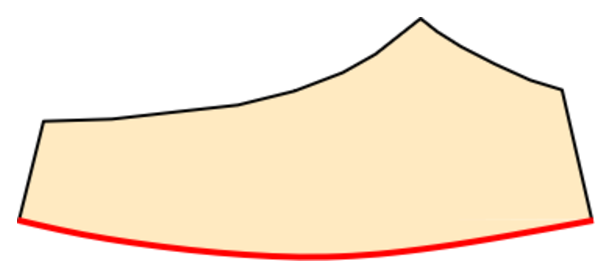
\includegraphics[width=0.45\columnwidth]{./figure/UpperPattern.eps}
		\label{fig:pattern_U}
	}
	\hfil
	\subfigure[lower pattern]{
		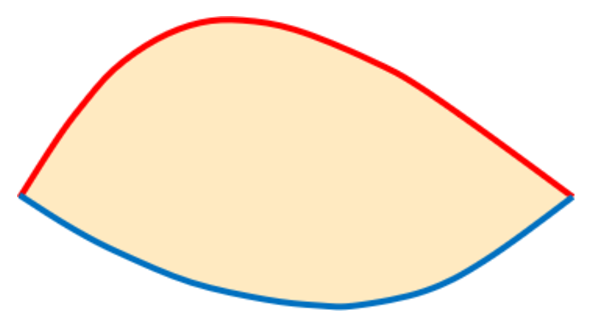
\includegraphics[width=0.45\columnwidth]{./figure/LowerPattern.eps}
		\label{fig:pattern_L}
	}
	\\
	\subfigure[lower line]{
		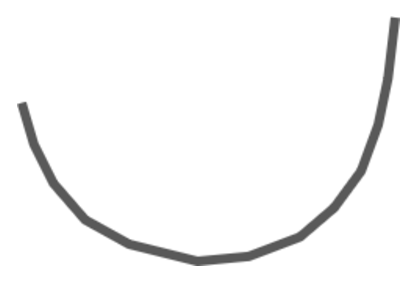
\includegraphics[width=0.35\columnwidth]{./figure/LowerWire.eps}
		\label{fig:Wire}
	}
	\caption{Parts of a two-piece brassiere cup}
	\label{fig:patterns}
\end{figure}
 And the cup has three curves and they are also very important to design. As shown in \rfig{fig:TwoCurves}, one is the wire line corresponding to the boundary between a breast and a body. Another is the ridge line of the cup corresponding to the outline of a bust on a transverse plane. The other is the upper line to connect a cup and shoulder strap. 

%==============================================================%
In apparel industries, the form of a product is fixed by fashion designers and pattern makers. Fashion designers draw an image of the product and pattern makers determine the shapes of patterns to meet various demands of the ideal shape, which previously mentioned about a brassiere, and so on.
%%fig
\begin{figure}[h!]
	\centering
	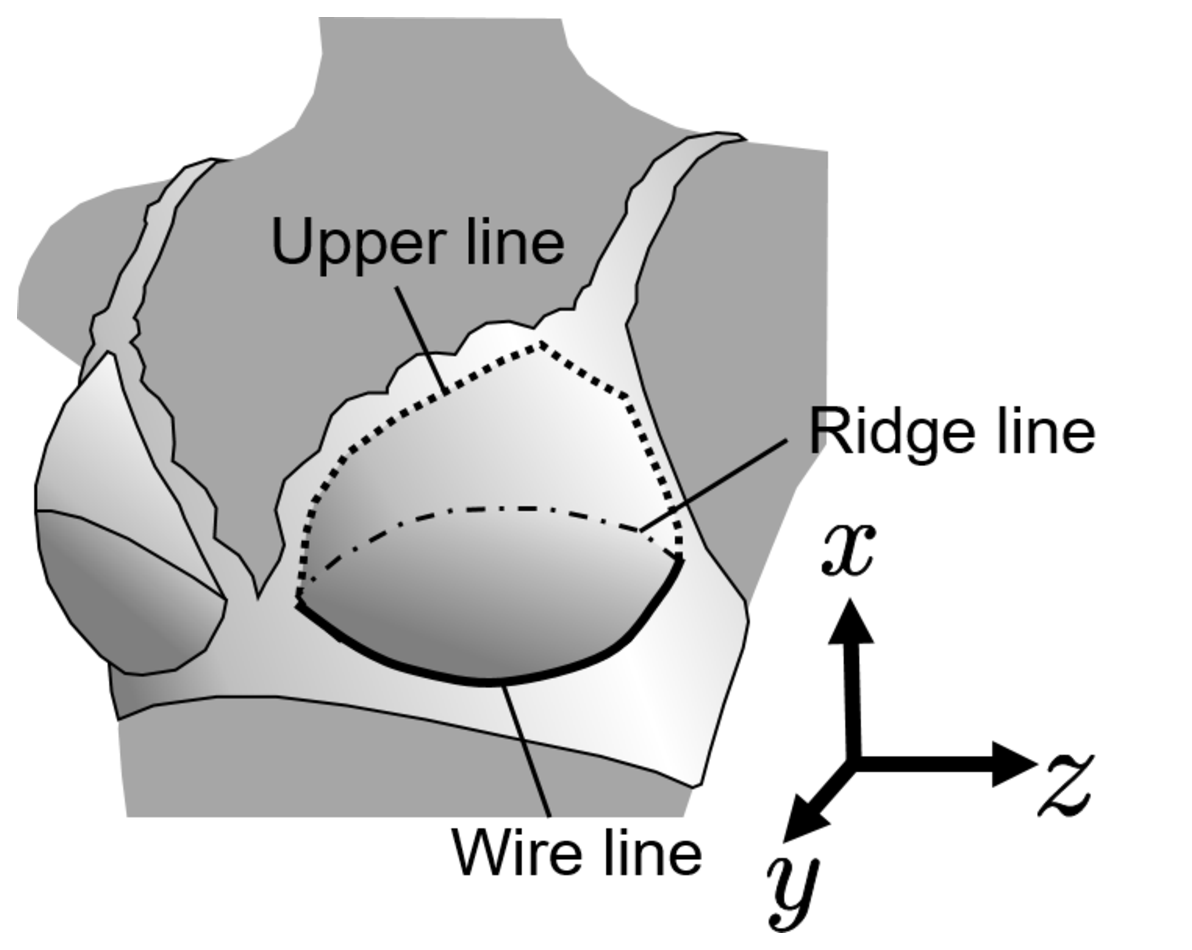
\includegraphics[scale=0.25]{./figure/Lines.eps}
	\caption{Expression of a wire line, a ridge line and an upper line}
	\label{fig:TwoCurves}
\end{figure}
The design process of a brassiere cup is shown in \rfig{fig:process}. In design cite, pattern makers first consider the functional requirement of a brassiere cup based on a breast shape, then determine the pattern shape. Since this design procedure cannot mainly be performed by CAD system but based on experience and intuition, they must check the shapes with a paper model of the cup and modify them repeatedly to realize the function. So, the situation may cause unnecessary repetition of modifying and checking pattern shapes. In order to improve the design efficiency of brassieres, it is required to reduce such trial and error as much as possible. So, in this paper, we focus on the process srrounded by a dotted line in \rfig{fig:process} and aim to automate it. 
When it comes to the function of a brassiere cup, Higuchi researched what emphasis is placed on in design of a brassiere cup\cite{c1}. According to  \cite{c1}, the function: fitting breast is most important. Therefore, we propose a method to design the shapes of patterns of a brassiere cup fitting the given breast shape. The given three-dimensional breast shape is assumed to be given as a cloud of data points, which can be obtained easily by measurement.

\begin{figure}[h!]
	\centering
	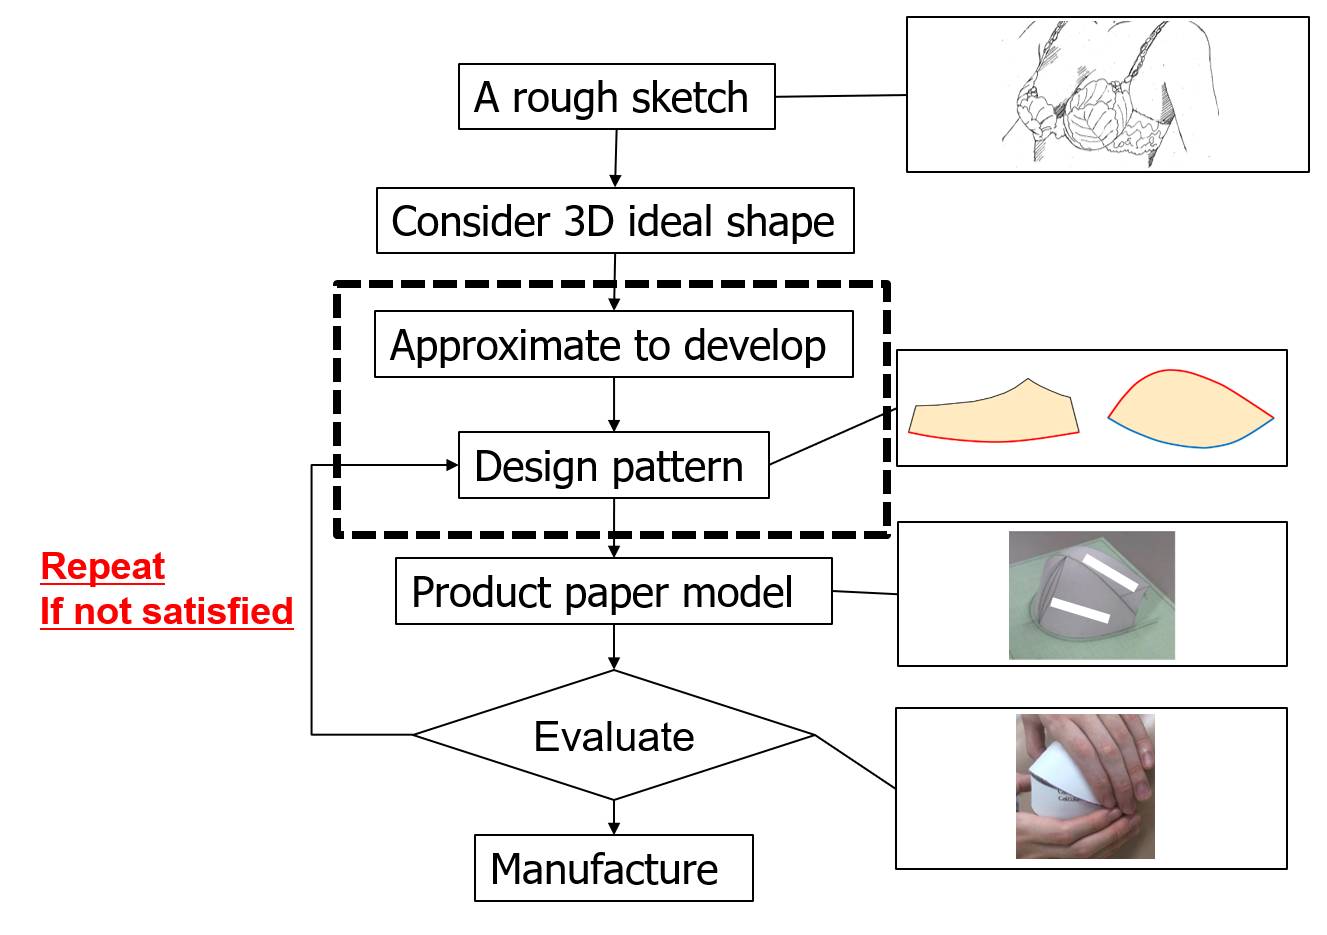
\includegraphics[width= 1.0 \columnwidth]{./figure/DesignProcess2.eps}
	\caption{Design process of a brassiere cup}
	\label{fig:process}
\end{figure}

%==============================================================%

As a cup shape is made by bending and sewing each pattern and assumed to be inextensible, the cup model consists of several developble surfaces.
With respect to modeling of develoable surfaces, a method to model developable surface by focusing on the geodesic line\cite{c2}, B-spline or NURBS surface\cite{c3,c4}, offsets of Bartrand curves which coincide each normal direction\cite{c5,c6}, and arbitrary curves on it\cite{c7}. Especially, Martin proposed a method to reconstruct developable surface from its point clouds based on Laguerre geometry\cite{c8}. Also, Chen et al. proposed an algorithm to approximate developable surface from its point cloud\cite{c9}. However, all of them does not reference its developed shape and only focus on a single developable surface. When it comes to manufacturing a brassiere cup, the pattern shapes, i.e. developed shapes of a cup is required, not 3D cup shape. Especially in a study on brassieres, Wakamatsu et al. proposed a method to predict the three-dimensional shape of a paper cup model when the two-dimensional shape of pattern is given \cite{c10,c11}. As a result, evaluation of the patterns becomes possible without actually creating a paper model. However, repetitive modification of the patterns is still required to obtain the target three-dimensional shape of the cup.
Ito et al. developed a paper model CAD system based on the theory of developable surfaces\cite{c12}. If a three-dimensional curve that means a sewn curve and a two-dimensional curve that means a piece to be sewn are given, a feasible region where the sewn surface does not intersect itself can be shown with this system. However, it is difficult to design the shape of patterns, that is, the shape of two-dimensional curves with this system.
We previously proposed method to design pattern shape and its developable surface from two lines: a wire line and a ridge line. They are obtained by solving optimization problem whose design parameters are the geodesic curvatures of a pattern shape and objective function is the error between generatrices determined by the geodesic curvature of a lower edge and the wire line and generatrices determined by the geodesic curvature of an upper edge and the ridge line. However, when it apply to this problem, it is required to  solve this optimization problem until the intended shape\cite{MyRef}. It leads to taking unnecessary time.
%==============================================================%


The products are mainly composed of two or three pieces of pattern. In this paper, we focus on two-piece brassiere cup and aim to propose a method to design its pattern shapes toward improvement of its design efficiency when a cloud of its data points is given.


%%%%%%%%%%%%%%%%%%%%%%%%%%%%%%%%%%%%%%%%%%%%%%%%%%%%%%%%%%%%%%%%%%%%%%
\section*{MODELING OF DEVELOPABLE SURFACE AND PATTERN SHAPE}

In this section, we aim to explain numerical expression of a developable surface. 
When it comes to a curvature of a space curve on a surface, it is divided to the normal curvature by deforming the surface and the geodesic curvature by deforming a space curve. The geodesic curvature does not change by deforming the surfce as long as it is not stretched. In case of a brassiere cup, the normal curvature can be manipulated by deforming the surface, but the geodesic curvature cannot. So, it is required to design the geodesic curvature in order to coincide a space curve with a boundary of the developable surface. Let \textit{lower edge} be the curve connecting to a lower wire as shown Fig.\ref{fig:pattern_L}, and \textit{upper edge} be the curve combining with upper cup as shown Fig.\ref{fig:pattern_L}. In this section, we aim to propose a method to determine a developable surface by two curves that lie on it and to design the pattern shape from them. We explain the method to express the developable surface from parameters of a space curve , the condition of two lines that lie on the developable surface, and a pattern shape obtained from them.
For this aim, we set object coordinate system on the lower edge of the cup surface as shown \rfig{fig:obj_coord} so that $\zeta$ -axis always coincides the tangential direction of the edge line and $\eta$ -axis always coincides the normal direction of the surface. The posture of the object coordinate system is changed by deformation of the cup. Then, the infinitesimal displacement vector of each axial direction can be described by the infinitesimal rotational ratio vector $ \mbold{\omega} = \left[\omega_{\xi}\;\;\omega_{\eta}\;\;\omega_{\zeta}\right]^{\mathrm{T}}$as follows:

\begin{equation}\label{eq:ObjSys}
\left[\begin{array}{ccc} \xivec' & \etavec' & \zetavec' \end{array}\right] = \left[\begin{array}{ccc} \xivec & \etavec & \zetavec \end{array} \right] \mbold{\Omega}(\mbold{\omega}), 
\end{equation}
where a prime means a derivative of $s$, and $\mbold{\Omega}(\mbold{\omega})$ is represented as follows: 
\begin{equation}
\mbold{\Omega}(\mbold{\omega}) = \left[\begin{array}{ccc}
0 &-\omega_{\zeta} & \omega_{\eta} \\
\omega_{\zeta} & 0 &-\omega_{\xi} \\
-\omega_{\eta} & \omega_{\xi} &0
\end{array}\right]. 
\end{equation}

Then, the tangent vector is expressed as follows: 
\begin{equation}
\zetavec(s) = \zetavec_0 + \int_{0}^{s} \left( \omega_{\eta} \xivec - \omega_{\xi} \etavec \right) ds,
\label{eq:zetav_eq}
\end{equation}
where $\zetavec_0$ represents the tangent vector at $s=0$ and by integrating \req{eq:zetav_eq}, the position of the curve can be calculated as follows:
\begin{equation}
\mbold{x}(s) = \mbold{x}_0 + \int_0^s \zetavec ds, 
\end{equation}
where $\mbold{x}_0$ means the position at $s=0$. 

\begin{figure}[thpb]
	\centering
	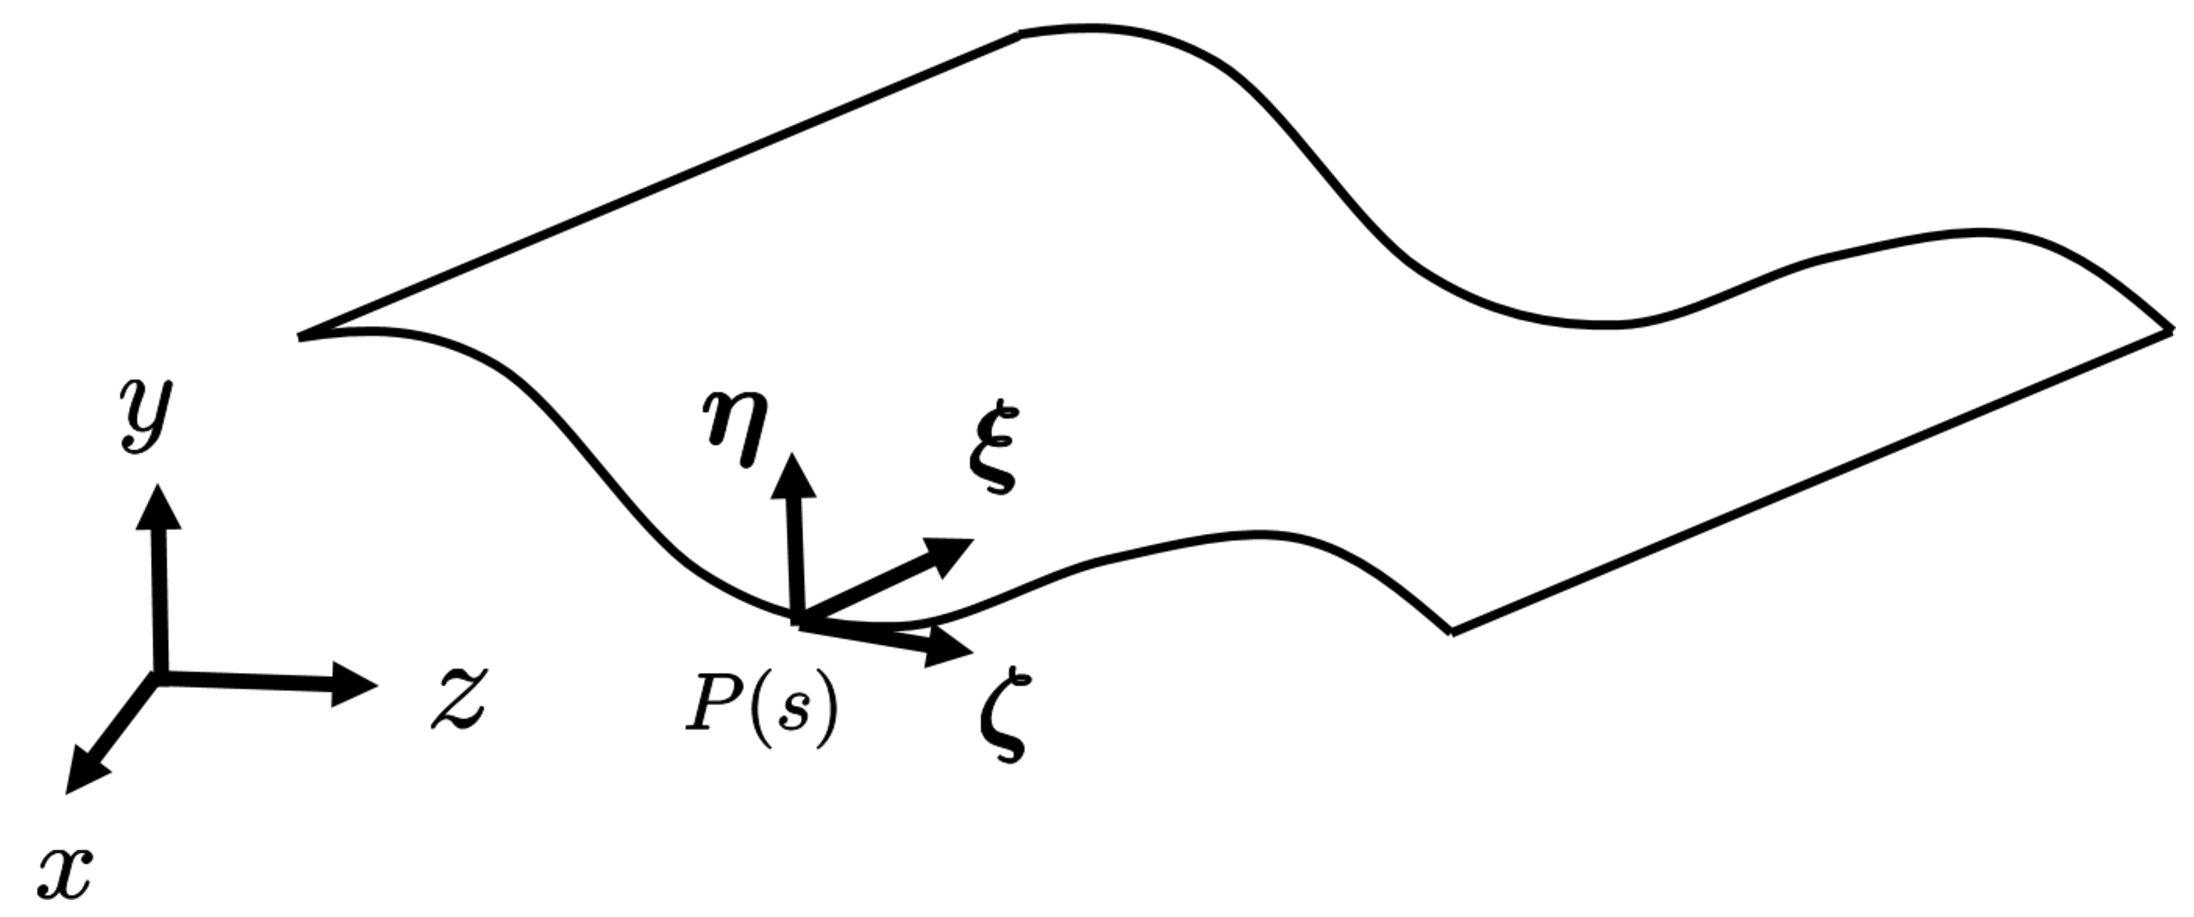
\includegraphics[width = 0.8\columnwidth]{./figure/Object_Coordinates.eps}
	\caption{Object coordinate system on the surface}
	\label{fig:obj_coord}
\end{figure}

First, we explain numerical expression of developable surface by the constraint of Gaussian curvature. 
In general, a normal curvature of a direction vector $\mbold{d}_{\theta} = \zetavec \cos \theta + \xivec \sin \theta $ can be described using coefficients of the first and the second fundamental forms $E, F, G, L, M$ and $N$:
\begin{equation}\label{eq:def_kappa_theta}
\kappa_{\theta} = \frac{L \cos^2 \theta + 2M \sin \theta \cos \theta + N \sin^2 \theta}{E \cos^2 \theta + 2F \sin \theta \cos \theta + G \sin^2 \theta}.
\end{equation}
And the Gaussian curvature $K$ and the mean curvature $H$, which characterize a surface, can be defined as extreme values of \req{eq:def_kappa_theta}: $ \kappa_{\max} $ and $ \kappa_{\min} $ as follows

\begin{eqnarray}
K &=& \kappa_{\max}  \kappa_{\min}  = \disfrac{LN-M^2}{EG-F^2}, \nonumber \\ 
H &=& \disfrac{\kappa_{\max} + \kappa_{\min}}{2} = \frac{EN-2FM+GL}{2(EG-F^2)}. 
\end{eqnarray}

In this paper, coefficients of first fundamental form are represented as following equation:
\begin{equation}
E = \zetavec \cdot \zetavec = 1, F = \zetavec \cdot \xivec = 0, G = \xivec \cdot \xivec = 1.
\end{equation}
Also, coefficients of second fundamental form are represented as following equation:
\begin{equation}
L = \zetavec' \cdot \eta = -\omega_{\xi}, M = \xivec' \cdot \eta = -\omega_{\zeta}.
\end{equation}
Then, Gaussian curvature $K$ and the mean curvature $H$ are described by
the following equation:

\begin{eqnarray}
\label{eq:GC_expressed_omega}
K &=& -\omega_{\xi} N - \omega_{\zeta}^2, \\
H &=& \disfrac{-\omega_{\xi}+N}{2}.
\end{eqnarray}
Developable surface is defined as the surface whose Gaussian curvature $K = 0$, which means $\kappa_{\min}=0$. Then, the mean curvature can be calculated as $2H=\kappa_{\max}$. This means that a line direction of which coincides with direction $\mbold{d}_{\min}$ is kept straight after deformation. This straight line is referred to as a generatrix. 
In this paper, principal directions are described by using the angle $ \alpha $: 
\begin{eqnarray}\label{eq:d1d2_eq}
\mbold{d}_{\max} &=& \zetavec \cos \alpha + \xivec \sin \alpha, \nonumber \\ 
\mbold{d}_{\min} &=& -\zetavec \sin \alpha + \xivec \cos \alpha.
\end{eqnarray}
The angle $ \alpha $ is referred to as the \textit{rib angle} in this paper.
By solving $ \kappa_{\theta} = 0 $, the rib angle $ \alpha $ can be calculated as following equation:
\begin{equation}\label{eq:alpha_eq}
\tan \alpha = -\frac{\omega_{\zeta}}{\omega_{\xi}}.
\end{equation}
And from \req{eq:GC_expressed_omega}, $\kappa_1$ is calculated as follows: 
\begin{equation}\label{eq:kappa1_eq}
\kappa_1 = -\frac{\omega_{\xi}^2 + \omega_{\zeta}^2}{\omega_{\xi}}.
\end{equation}
From above, a developable surface can be determined by $\mbold{\omega}$.
%%%%%%%%%%%%%%ここまで7/21

Next, we explain the constraint of developable surface when two curves that lie on the surface are given. Let $s_a$ and $s_b$ be the arc length and $\mbold{x}_a(s_a)$, $\mbold{x}_b(s_b)$ be positions of each curve. We assume that these curves have ${\rm C}^2$ community at least. In general developable surfaces are a special kind of ruled surfaces. When the surface is a ruled surface, a generatrix $ \mbold{g} $ is described as follows:

\begin{equation}
\mbold{g} = \mbold{x}_b(s_b)-\mbold{x}_a(s_a).
\end{equation}

Note that $s_a$ can take an arbitrary value against $ s_b $. Therefore, the variation of a generatrix $ \Delta \mbold{g} $ is described by total differential form as follows:
\begin{equation}
\Delta \mbold{g} = -\zetavec_a \Delta s_a + \zetavec_b \Delta s_b,
\end{equation}
where $ \zetavec_a$ and $\zetavec_b $ are tangent vectors of $ \mbold{x}_a $ and $ \mbold{x}_b $, respectively. Next, let $ \Theta $ be the infinitesimal plane surrounded by four vectors $ \zetavec_a \Delta s_a, \zetavec_b \Delta s_b,\mbold{g}$, and $\mbold{g}+\Delta \mbold{g} $ as shown in \rfig{fig:Theta}. When the ruled surface is a developable surface, the plane $ \Theta $ is a tangent plane without twisting. Therefore, it leads to following equation:
\begin{equation}
\det (\zetavec_a, \mbold{g}, \mbold{g}+\Delta \mbold{g})=0
\end{equation}
By solving it, the following equation is obtained:
\begin{equation}
\det (\zetavec_a, \zetavec_b, \mbold{g})=0
\label{eq:Cond1}
\end{equation}
\begin{figure}[!h]
	\centering
	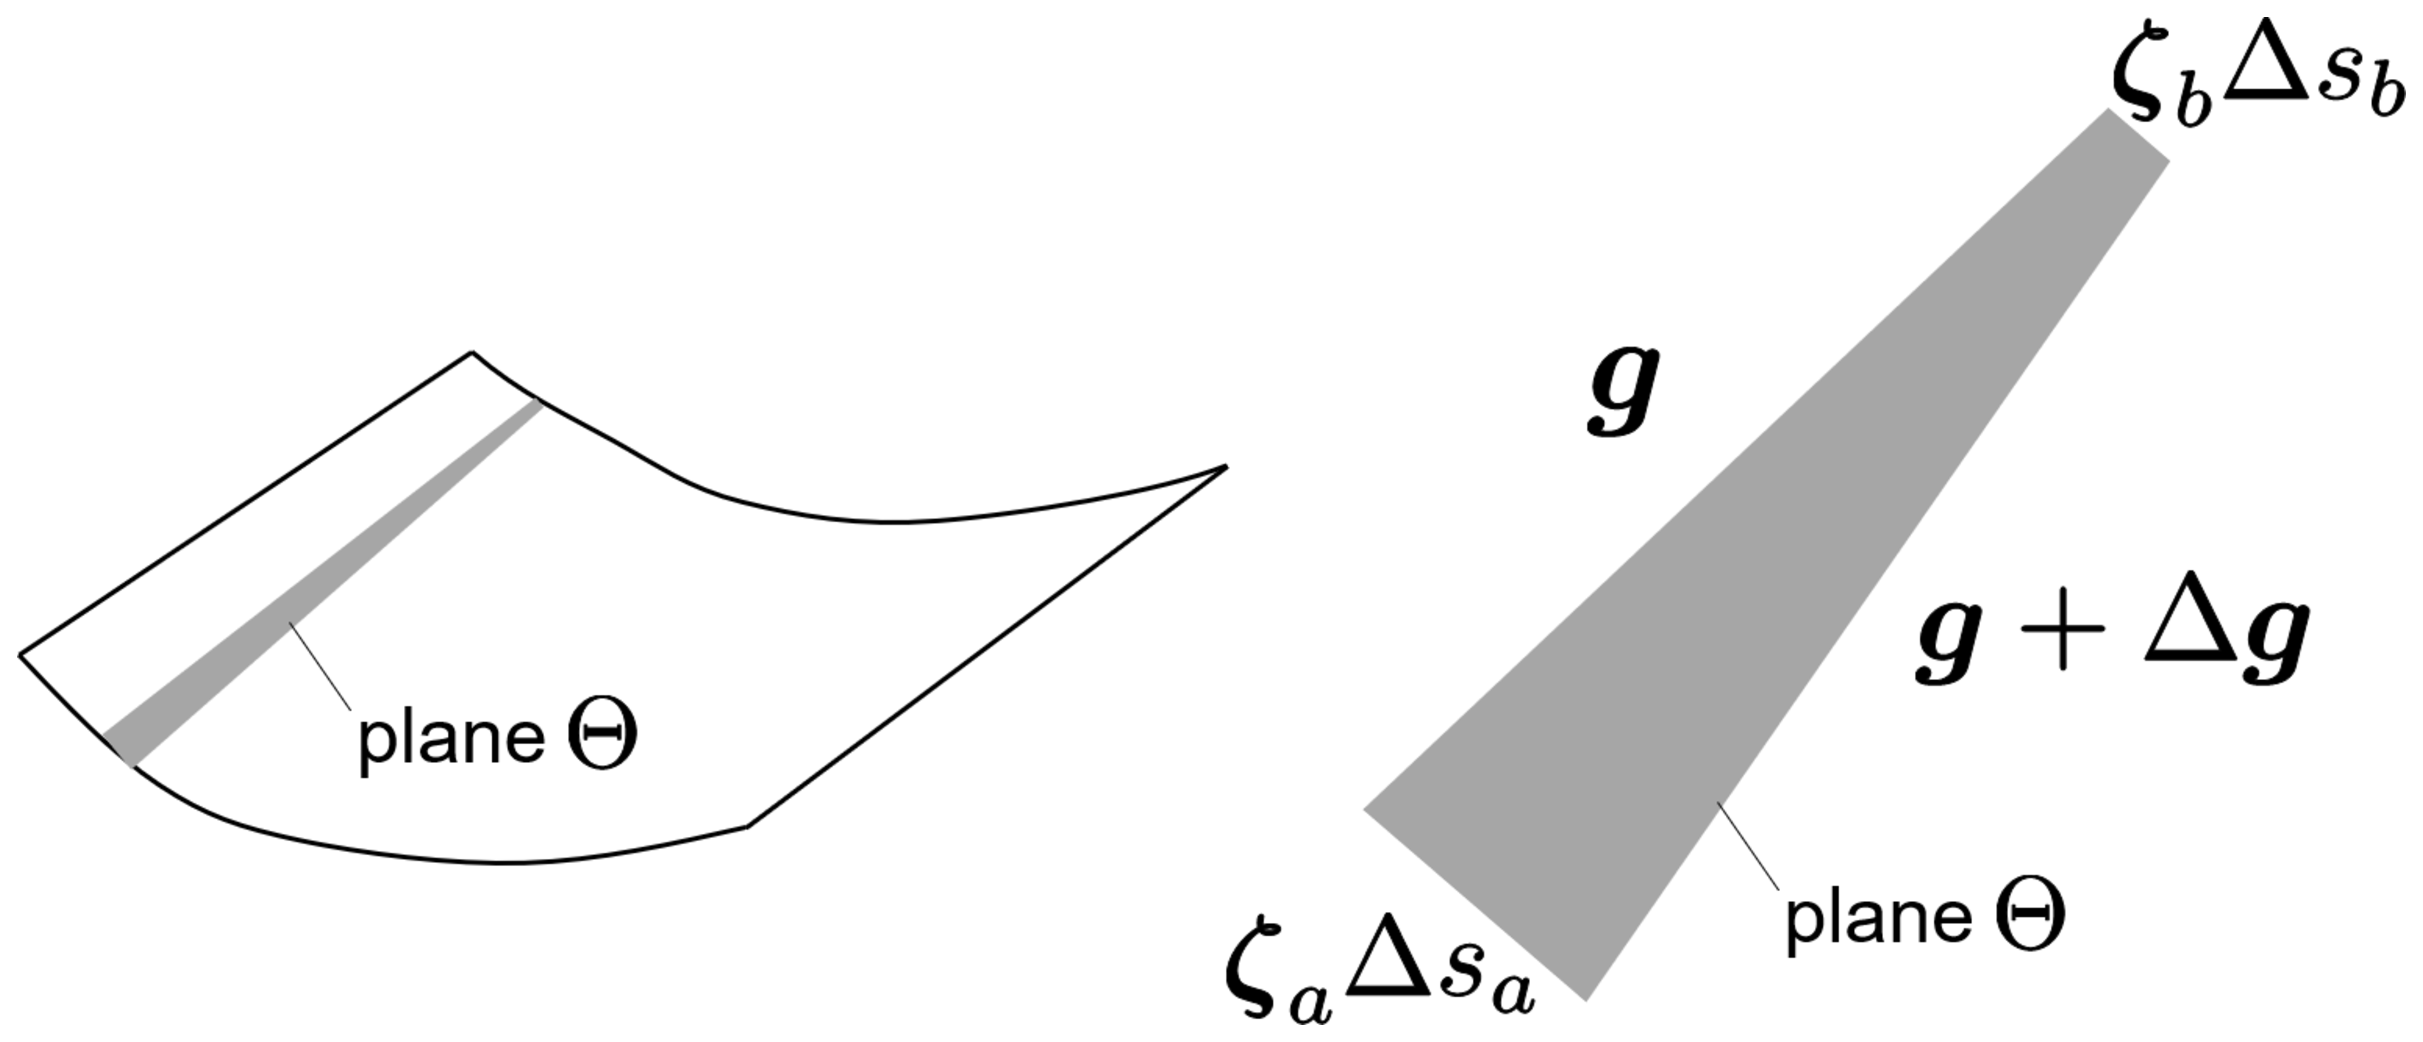
\includegraphics[width = 0.8\columnwidth]{./figure/Theta.eps}
	\caption{Definition of $ \Theta $}
	\label{fig:Theta}
\end{figure}
It indicates that the arc length of each curve is subordination. When two curves are corresponded to edge lines and $s_b$ can be expressed as $s_b(s_a)$, $\mbold{d}_{\min}\equiv\frac{\mbold{g}}{|\mbold{g}|}$ is established. Then, a rib angle is calculated by \req{eq:d1d2_eq} as follows:
\begin{equation}
\alpha = -\sin^{-1}\left( \mbold{d}_{\min} \cdot \zetavec_a \right).
\end{equation}
Using $\mbold{d}_{\min}$ and $\alpha$, $\mbold{\omega}$ can be represented as following equation:
\begin{equation}\label{eq:omegaVec}
\mbold{\omega} = \left[\begin{array}{c} -\det(\zetavec_a',\zetavec_a, \mbold{d}_{\min} ) \\ \zetavec_a' \cdot \mbold{d}_{\min} \\ \det(\zetavec_a',\zetavec_a, \mbold{d}_{\min} ) \tan \alpha \end{array}\right] 
\end{equation}
Therefore, when two curves that lie on the surface are given, a developable surface can be determined.

Next, we explain how to determine the pattern shape from the developable surface. The planar curve generated by developing the space curve $ \mbold{x}_a $ is defined a the lower curve and that by developing the space $ \mbold{x}_b $ is defined as the upper curve.

We set developed planar coordinate system $ vw $ so that $ v $-axis always coincides the line AB as shown in \rfig{fig:PatternImage}. Let $ \mu_a $ be the angle between the tangential direction of the lower edge and the $ v $-axis. $ \mu_a $ is obtained as follows when the curvature of the lower curve $ \omega_{\eta_a} $  is given:
\begin{equation}\label{eq:mu_eq}
\mu_a = \mu_0 + \int_{0}^{s_a} \omega_{\eta_a} ds_a,
\end{equation}
where $ \mu_0 $ represents the angle of the lower edge at $ s=0 $ and is described later. From \req{eq:mu_eq}, the planar position $ \mbold{x}_{ae} $ is described as follows:
\begin{equation}\label{eq:x_LE}
\mbold{x}_{ae}  = \int_{0}^{s_a} \left[\begin{array}{cc} \cos \mu_a \\ \sin \mu_a \end{array}\right] ds_a
\end{equation}
With respect to \req{eq:mu_eq}, let $ a,b $ be defined as follows:
\begin{eqnarray}
a &=& \int_{0}^{L_a} \cos \left( \int_{0}^{s_a} \omega_{\eta_a} ds\right) ds_a, \\
b &=& \int_{0}^{L_a} \sin \left( \int_{0}^{s_a} \omega_{\eta_a} ds\right) ds_a. 
\end{eqnarray}
Then, $ \mu_0 $ can be calculated as follows:
\begin{equation}\label{eq:mu_0eq}
\mu_0 = \tan^{-1}\frac{b}{a}
\end{equation}
Let $ \mbold{x}_{be} $ be the planar position of an upper edge. Since the rib angle of a pattern $ \alpha_a $ and the length of a generatrix of a pattern $ |\mbold{g}| $ don't change by being developed, $ \mbold{x}_{be} $ can be calculated as follows:
\begin{equation}\label{eq:x_UE}
\mbold{x}_{be} = \mbold{x}_{ae} + |\mbold{g}| \left[\begin{array}{cc} \cos \left(\mu_a + \pi/2 + \alpha_a \right) \\ \sin \left(\mu_a + \pi/2 + \alpha_a \right)  \end{array}\right] 
\end{equation}
From above, a developed shape can be obtained when two curves that lie on the developable surface are given.
\begin{figure}[thpb]
	\centering
	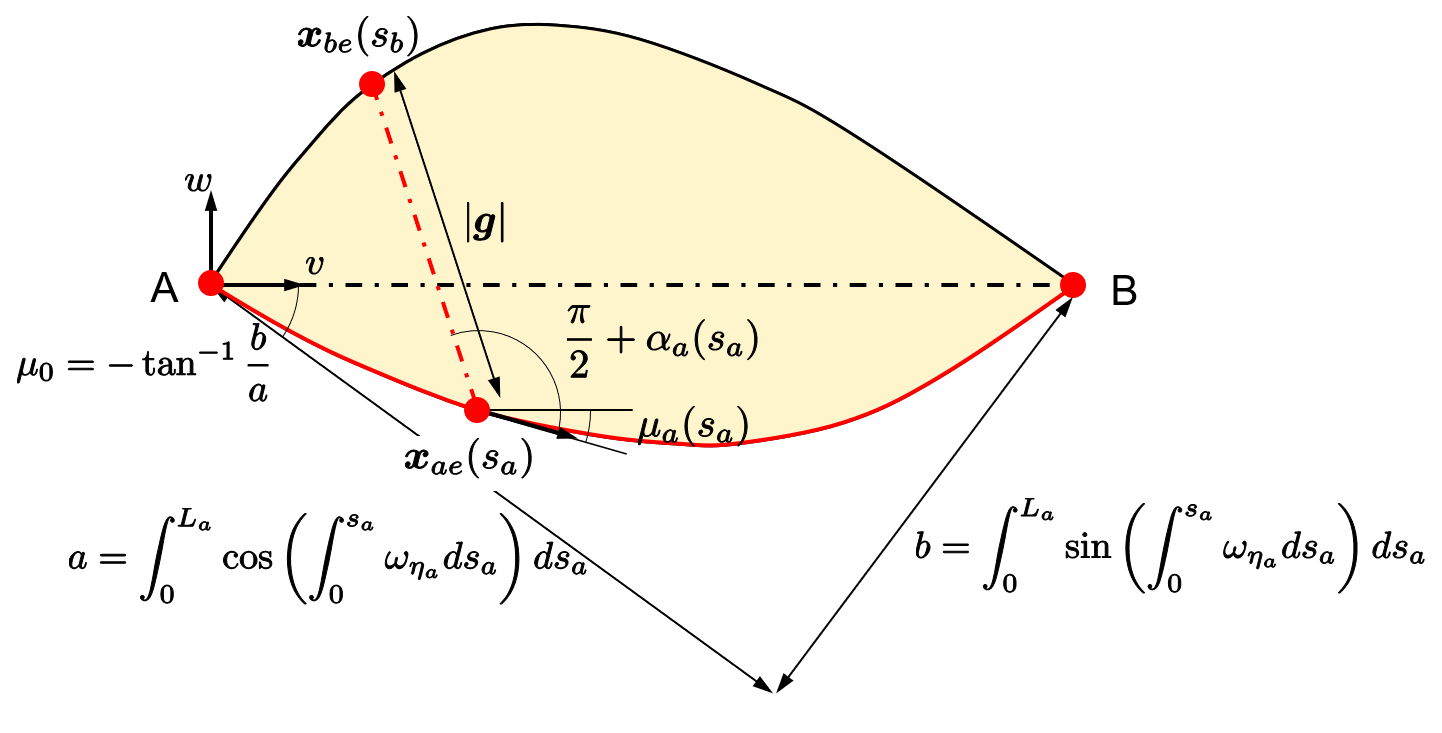
\includegraphics[width = \columnwidth]{./figure/PatternImage2.eps}
	\caption{Description of pattern shape using geodesic curvature of the lower curve}
	\label{fig:PatternImage}
\end{figure}
\section*{EXPRESSION OF DESIGN PROCESS AS OPTIMIZATION PROBLEM}
From section2, the cup shape can be determined by three curves: a wire wire, a ridge line and an upper line. Therefore, when a wire line is given, the objective of our study can be achieved by designing parameters of a ridge line and an upper line, which minimize the degree of fitting to the 3D breast shape. So, in this section, we aim to formulate this degree. 
%%%%%%%%%%%%%%%%%%%%%%%%%%%%%%%%%%%%%%%%%%%%%%%%%%%%%%%%%%%%%%%%%%%%%%
\subsection*{Formulation of the error between a point and a surface}
In order to formulate the degree of fitting to the 3D ideal shape, we formulate the error between a point and a surface.
In general, the position $\mbold{X}(s,t)$ of developable surface $S$ is expressed as following equation:
\begin{equation}\label{eq:Sur_eq}
\mbold{X}(s,t) = \mbold{x}(s) + t\mbold{d}_{\min}(s)
\end{equation}
The distance $\varepsilon(\mbold{p})$ between a point $\mbold{p}$ and a developable surface is formulated by the difference vector $\mbold{\delta}=\mbold{p}-\mbold{X}(s,t)$ as follows:

\begin{equation}\label{eq:eps_eq}
\varepsilon(\mbold{p})=\min_{s,t}{|\mbold{\delta}|}
\end{equation}

When a set of surface parameters $ (s^*,t^*) $ satisfies to minimize \req{eq:eps_eq}, $\mbold{\delta}$ is parallel to $ \etavec $. Therefore, the following equations are satisfied:
\begin{equation}\label{eq:d_mindoteq}
\mbold{d}_{\min} \cdot (\mbold{p} - \mbold{X}(s^*,t^*)) = 0
\end{equation}

\begin{equation}\label{eq:d_maxdoteq}
\mbold{d}_{\max} \cdot (\mbold{p} - \mbold{X}(s^*,t^*)) = 0
\end{equation}
By solving \req{eq:d_mindoteq}, $ t^* $ is described as follows:

\begin{equation}\label{eq:t*_eq}
t^* = \mbold{d}_{\min} \cdot (\mbold{p}-\mbold{X}(s^*))
\end{equation}
By using \req{eq:t*_eq} and solving \req{eq:d_maxdoteq}, $ s^* $ is determined.

Let $ s_w,s_r,s_u $ be arc lengths of a lower wire, ridge line, and upper line and $ \mbold{\omega}_W (s_w ),\mbold{\omega}_R (s_r ),\mbold{\omega}_U (s_u ) $ be vectors to characterize each of them. From \req{eq:Cond1}, $ s_r,s_u $ can be expressed as functions of $ s_w $: $ s_r (s_w ),s_u (s_w ) $. As mentioned, a two-piece brassiere cup is composed of two developable surfaces $ S_L $ and $ S_U $. Let $ D $ be the set of coordinates of points on a breast, $ D_L = \{\mbold{p}_{L,i} \in D \} $ be the set of points to evaluate the surface $ S_L $, and $ D_U = \{\mbold{p}_{U,i} \in D \} $ be the set of points to evaluated the surface $ S_U $, respectively. Note that $ D_U = D \backslash D_L $. Whether a point $ \mbold{p}_k $ is classified to the set of $ D_U $ or the set of $ D_L $ can determined with the length of the nearest generatrix.

First, \req{eq:d_mindoteq,eq:d_maxdoteq,eq:t*_eq}, the nearest surface parameters $ (s_w^*, t_w^*) $ of the lower cup to the point $ \mbold{p}_k $ can be derived. Then, the nearest point $ \mbold{X}(s^*, t^*) $ on the lower cup surface to the point $ \mbold{p}_k $ can be derived. Let $ t_{\max}=|\mbold{x}_R (s_r (s_w^* ))-\mbold{x}_W (s_w^* )| $ be the length of a generatrix on the wire line. If $ t_{\max} > t_w^*(s_w^*) $, that is, if the perpendicular projection point of the point $ \mbold{p}_k $ to the surface $ S_L $ is included in the lower cup, the point $ \mbold{p}_k $ is classified to the set $ D_L $. Otherwise, it is classified to the set $ D_U $. 
\begin{figure}[thpb]
	\centering
	\subfigure[$ t^*\leq t_{\max} $]{
		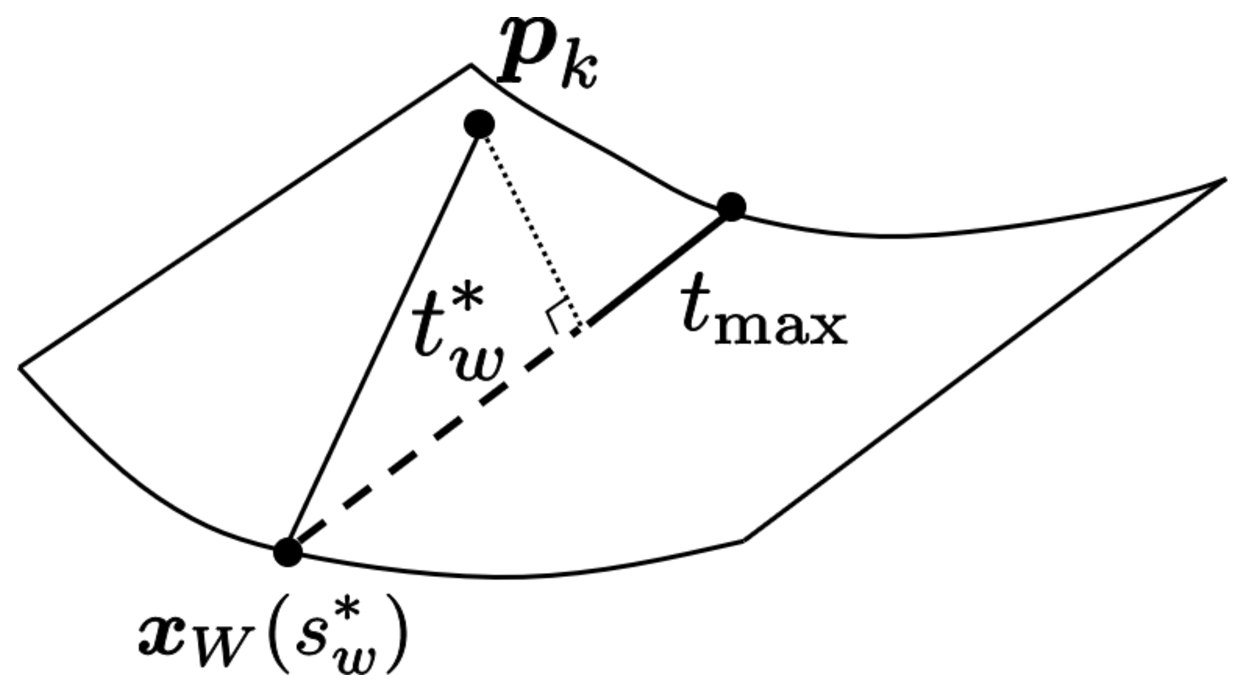
\includegraphics[width=0.45\columnwidth]{./figure/NotExceeding.eps}
		\label{fig:inD_L}
	}
	\hfil
	\subfigure[$ t^* > t_{\max} $]{
		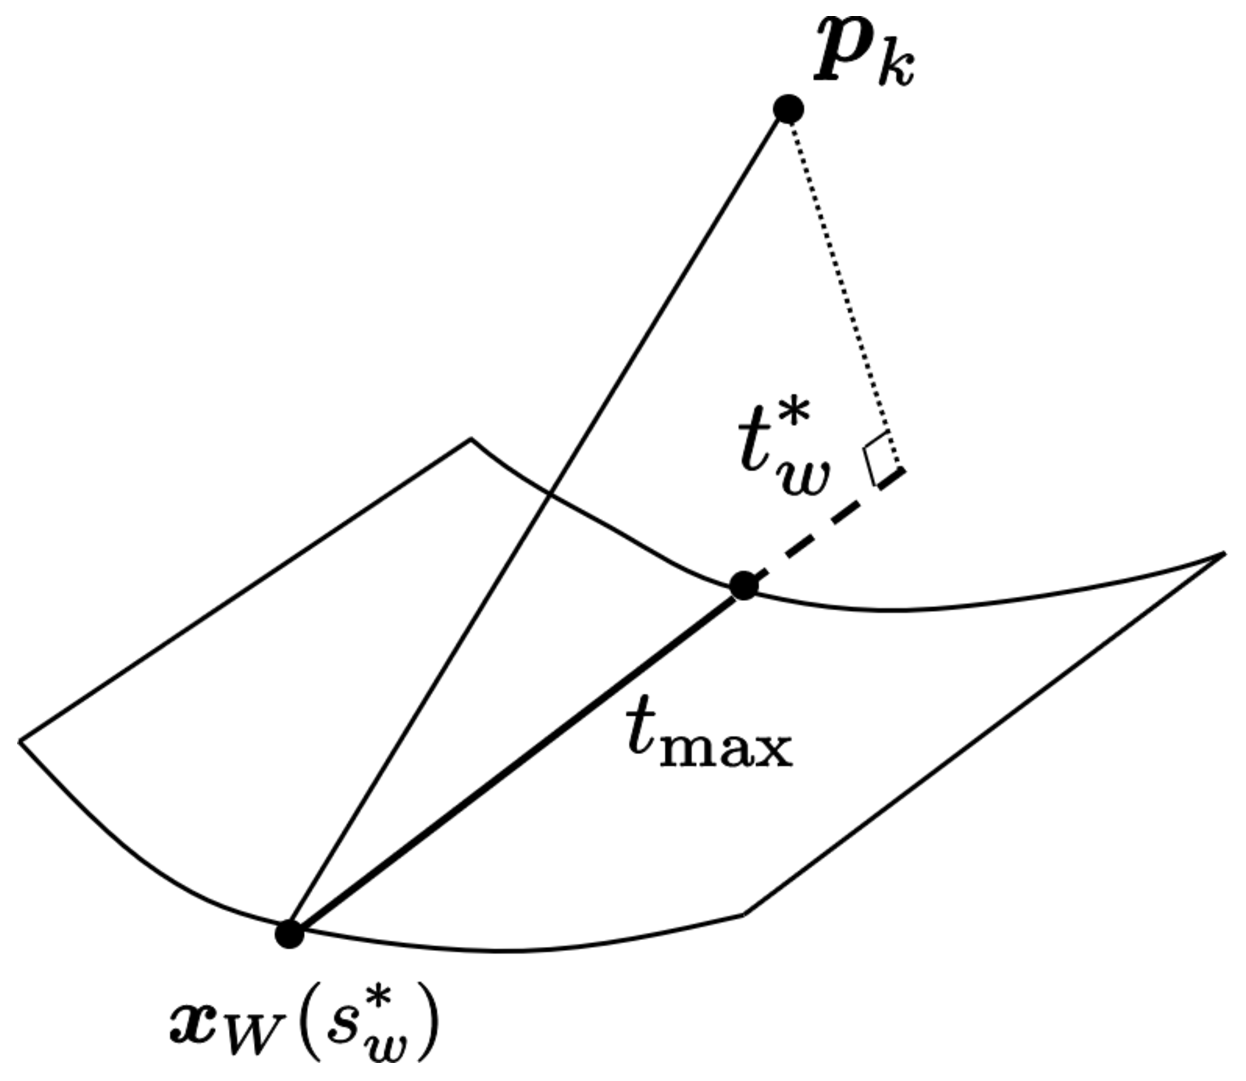
\includegraphics[width=0.45\columnwidth]{./figure/Exceeding.eps}
		\label{fig:inD_U}
	}
	\caption{Relationship between $ t^*$ and $t_{\max}$.}
	\label{fig:which_in}
\end{figure}

Thus, we can classify point data on a breast into two sets once two developable surfaces for the lower and the upper cup are determined.

From above, the error between the surface of a two-piece brassiere cup and its data points can be formulated:
\begin{equation}\label{eq:Lambda_eq}
\Lambda(D) = \sum_{i=1}^{N_L} \varepsilon(\mbold{p}_{L,i}) + \sum_{i=1}^{N_U} \varepsilon(\mbold{p}_{U,i}).
\end{equation}
By finding two developable surfaces minimizing the error described by \req{eq:Lambda_eq}, appropriate pattern shapes can be determined.


\subsection*{Formulation of Objective Function and Conditions}
Let us consider the conditions of this optimization. First, we explain the conditions about parameters of the ridge line and the upper line. When it comes to designing the space curve, $ \omega_{\zeta} $ does not affect its shape. Therefore, the following conditions are added:
\begin{eqnarray}\label{eq:conds_omgZt}
\omega_{\zeta_R}(s_r(s_w)) &=& 0 \;\; \forall s_w\in[0,L_L], \\
\omega_{\zeta_U}(s_u(s_w)) &=& 0 \;\; \forall s_w\in[0,L_L]. 
\end{eqnarray}

When it comes to designing their arc length, the following  conditions  must be satisfied:
\begin{equation}\label{eq:conds_arc1}
	s_r(s_w) \geq 0 \;\; \forall s_w\in[0,L_L], 
\end{equation}
\begin{equation}\label{eq:conds_arc2}
	s_u(s_w) \geq 0 \;\; \forall s_w\in[0,L_L], 
\end{equation}
\begin{equation}\label{eq:conds_arc3}
	s_r'(s_w) \geq 0 \;\; \forall s_w\in[0,L_L], 
\end{equation}
\begin{equation}\label{eq:conds_arc4}
	s_u'(s_w) \geq 0 \;\; \forall s_w\in[0,L_L].
\end{equation}
In general, the end positions of the ridge line and the upper line are aligned to the end point of the wire line. Therefore, the following equations must be satisfied:
\begin{equation}\label{eq:conds_endp1}
	\mbold{x}_R (s_r(s_w)) = \mbold{x}_L(s_w), 
\end{equation}
\begin{equation}\label{eq:conds_endp2}
	\mbold{x}_U (s_u(s_w)) = \mbold{x}_L(s_w).
\end{equation}

In order to guarantee $ S_L $ and $ S_U $  are developable surfaces, the following equations must be satisfied:
\begin{equation}\label{eq:conds_DevSur1}
	\int_{0}^{L_L} \det (\zetavec_R(s_r(s_w)), \zetavec_W(s_w), \mbold{g}) ds_w = 0,
\end{equation}
\begin{equation}\label{eq:conds_DevSur2}
	\int_{0}^{L_L} \det (\zetavec_U(s_u(s_w)), \zetavec_W(s_w), \mbold{g}) ds_w = 0.
\end{equation}
Next, let us consider a “fuzzy” condition of a brassiere cup. 
The upper line has a point to be connected with a shoulder strap. In this paper, we call this point \textit{connection point}. In design process, this point is usually not given as a unique condition, but a fuzzy condition.
\begin{figure}[!h]
	\centering
	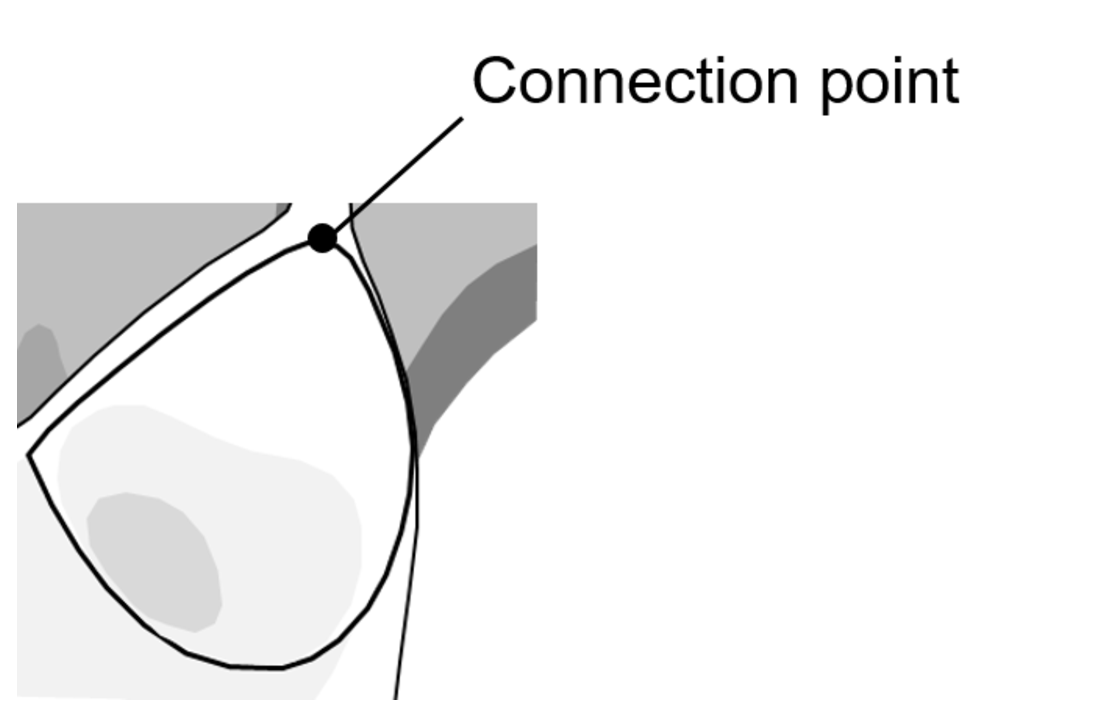
\includegraphics[width = 0.7\columnwidth]{./figure/Connection_Point.eps}
	\caption{Expression about the connection point of a brassiere cup}
	\label{fig:aboutCP}
\end{figure}
It may cause unexpected error of the optimization problem. Therefore, we propose the following equation to deal with this fuzzy condition $ y \simeq Y $:
\begin{equation}\label{eq:FuzzyEq}
C(y,Y) = k_1 \exp( k_2(y-Y)^2 )
\end{equation}
where $ k_1 $ and $ k_2 $ are the variables to adjust a range of satisfying this condition. By adding this equation to the objective function, the fuzzy condition can be dealt. In this paper, we assumed that the position $ \mbold{X}_C $ to connect the upper line and the shoulder strap is given. Then, the objective function $ V $ is described as follows:
\begin{equation}\label{eq:ObjectFunc}
V = \Lambda(\mbold{D}) + \sum_{i=0}^{2} C(\mbold{x}_U \cdot \mbold{e}_i , \mbold{X}_C \cdot \mbold{e}_i)
\end{equation}
where $\mbold{e}_0 $ ,$\mbold{e}_1 $ and $\mbold{e}_2 $ are represented as unit vectors of $ x $,$ y $ and $ z $-axis. By solving this optimization under the constraints, the shape of the brassiere cup, satisfying to fit data points of a breast, can be obtained.

\subsection*{A Procedure of Solving Optimization Problem}
Let us explain a procedure of solving this optimization problem. First, we explain how to eliminate the condition. In order to satisfy \req{eq:conds_arc1,eq:conds_arc2,eq:conds_arc3,eq:conds_arc4}, $ s_r (s_w),s_u (s_w) $ are described using arbitrary functions $ \upsilon_r(s_w),\upsilon_u(s_w) $ as follows:
\begin{eqnarray}
s_r(s_w) &=& s_{r_0} + \int_{0}^{s_w} \upsilon_r^2 ds_w, \\
s_u(s_w) &=& s_{u_0} + \int_{0}^{s_w} \upsilon_u^2 ds_w. 
\end{eqnarray}
When we assume that the initial position of the wire line, that of the ridge line, and that of the upper line are aligned, $ s_{r_0}=s_{u_0}=0 $. Let a composite function of $ s_r(s_w) $ and arbitrary function $ g(s_r) $ be defined as $ \tilde{g}(s_w) $, and a composite function of $ s_u (s_w ) $ and arbitrary function $ g(s_w) $ be defined as $ \hat{g}(s_w) $. Then, from \req{eq:ObjSys}, the object coordinate system of the ridge line and upper line can be expressed as follows:
\begin{equation}\label{eq:tildeobj}
\left[\begin{array}{ccc} \tilde{\xivec}_R' & \tilde{\etavec}_R' & \tilde{\zetavec}_R' \end{array}\right] = s_r' \left[\begin{array}{ccc} \tilde{\xivec}_R & \tilde{\etavec}_R & \tilde{\zetavec}_R \end{array} \right] \Omega(\tilde{\mbold{\omega}}_R)
\end{equation}

\begin{equation}\label{eq:hatobj}
\left[\begin{array}{ccc} \hat{\xivec}_U' & \hat{\etavec}_U' & \hat{\zetavec}_U' \end{array}\right] = s_u' \left[\begin{array}{ccc} \hat{\xivec}_U & \hat{\etavec}_U & \hat{\zetavec}_U \end{array} \right] \Omega(\hat{\mbold{\omega}}_U)
\end{equation}
and the position $ \mbold{x}_R(s_r) \equiv \tilde{\mbold{x}}_R(s_w) $ and $ \mbold{x}_U(s_u) \equiv \hat{\mbold{x}}_U(s_w) $ are expressed by the following equations:
\begin{eqnarray}
\tilde{\mbold{x}}_R(s_w) &=& \int_{0}^{s_w} \tilde{\zetavec}_R s_r' ds_w \\
\hat{\mbold{x}}_U(s_w) &=& \int_{0}^{s_w} \hat{\zetavec}_U s_u' ds_w
\end{eqnarray}

Let $ \mbold{\psi} = [\omega_{\xi} \;\; \omega_{\eta} \;\; \upsilon] $ be the function vector of a line. Then, the vector of the ridge line $ \mbold{\psi}_R $ and the vector of the upper line $ \mbold{\psi}_U $ are represented using Ritz method\cite{c13} as follows:
\begin{equation}\label{eq:R_eq}
\mbold{\psi}_R = \left[ \begin{array}{ccc} \mbold{a}_{\omega_{\xi_R}}& \mbold{a}_{\omega_{\eta_R}}& \mbold{a}_{\upsilon_R} \end{array} \right] \cdot \mbold{e}(s_w) = \mbold{a}_R \cdot \mbold{e}(s_w) 
\end{equation}

\begin{equation}\label{eq:U_eq}
\mbold{\psi}_U = \left[ \begin{array}{ccc} \mbold{a}_{\omega_{\xi_U}}& \mbold{a}_{\omega_{\eta_U}}& \mbold{a}_{\upsilon_U} \end{array} \right] \cdot  \mbold{e}(s_w) = \mbold{a}_U \cdot \mbold{e}(s_w)
\end{equation}
where $ \mbold{e}_i(s) $ is composed of trigonometric functions with different periods. And let $ \mbold{\Phi}_0 = [\xivec_0^\mathrm{T} \;\; \etavec_0^\mathrm{T} \;\; \zetavec_0^\mathrm{T}] $ be an initial basis of the objective coordinate system.

From above, the objective function expressed as \req{eq:ObjectFunc} and geometric constraints expressed as \req{eq:conds_endp1,eq:conds_endp2,eq:conds_DevSur1,eq:conds_DevSur2} are described by the following total parameter vector: 
\begin{equation}\label{eq:TotalCoefs}
\mbold{a}_{\mathrm{all}} = \left[ \begin{array}{cccc}
\mbold{a}_R & \mbold{a}_U & \mbold{\Phi}_{R0} &\mbold{\Phi}_{U0} 
\end{array}\right].
\end{equation}

Consequently, this problem can be converted to a non-linear programming problem. It is solved by the multiplier method and Nelder-Mead method in this paper. By solving the above problem, we can design the entire shape of a two-piece brassiere cup.

\section*{SIMULATION AND VERIFICATION}
In this section, we aim to consider the simulation result and verification of our proposed method. For this verification, the infinitesimal rotational ratios vector $ \mbold{\omega}_W $ of the wire line was given as follows:
\begin{equation}\label{eq:vrf_omgW}
\mbold{\omega}_W = \left[ \begin{array}{ccc}
0 & 2.91 & 0
\end{array}\right]^\mathrm{T}, 
\end{equation}
and, the connection point $ \mbold{X}_C $ was given as follows: 
\begin{equation}\label{eq:givenXc}
\mbold{X}_C = \left[ \begin{array}{ccc}
0 & 0.34 & 0.34
\end{array}\right]^\mathrm{T}.
\end{equation}
We prepared two examples of the simulation.

Case (1): a point cloud on the sphere whose radius is set on R by uniform random number. 

Case (2): a point cloud on the set of developable surface by uniform random number using \req{eq:Sur_eq}. 

And we aim to confirm two matters by them.
\begin{enumerate}
	\item to design the two-piece brassiere cup which can approximate undevelopable surface, which means it menifests the function: fitting to a breast".
	\item to recreate the same shape that of given shape.
\end{enumerate}
In this study, uniform random number was generated by numpy.random() of Pyhton. At first, we show the result in case(1).

As shown in \rfig{fig:ObtainedSurfaceNDS}, the solid line represents the given wire line, each dotted line does calculated generatrices of the cup shape, and each dots does the given data points. And the pattern shapes were calculated as shown in \rfig{fig:ObtainedSurfaceNDS_Pat}. In \rfig{fig:ObtainedSurfaceNDS_Pat}, each solid line represents a lower edge and a dotted line represents an upper edge. In this result, we could confirm that the designed cup shape by our proposed method menifests the function:"fitting to a breast".
Next, we show the result in case(2). In \rfig{fig:ObtainedSurfaceDS}, the solid line, each dotted line and dot represent as same as case(1). And the pattern shapes were calculated as shown in \rfig{fig:ObtainedSurfaceDS_Pat}. In \rfig{fig:ObtainedSurfaceDS_Pat}, a solid line and a dotted line represent as same as case(1).

As the calculated shapes approximate the given points, we conclude our proposed method in this paper is useful for efficient design of paper patterns of a two-piece brassiere cup.
\begin{figure}[h]
	\centering
	\subfigure[zx-view]{
		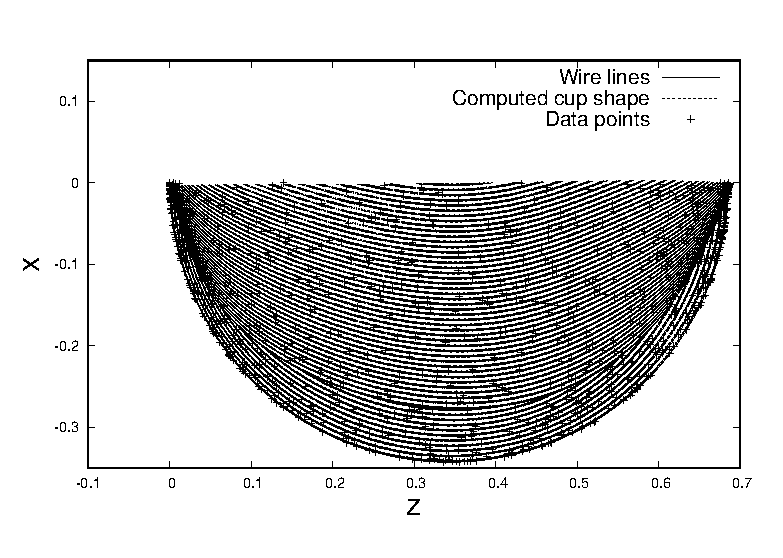
\includegraphics[width=0.6\columnwidth,clip]{./figure/NDS/ObtainedRidgeLinefromz-x.eps}
		\label{fig:zx-NDS}
	}
	\hfil
	\subfigure[zy-view]{
		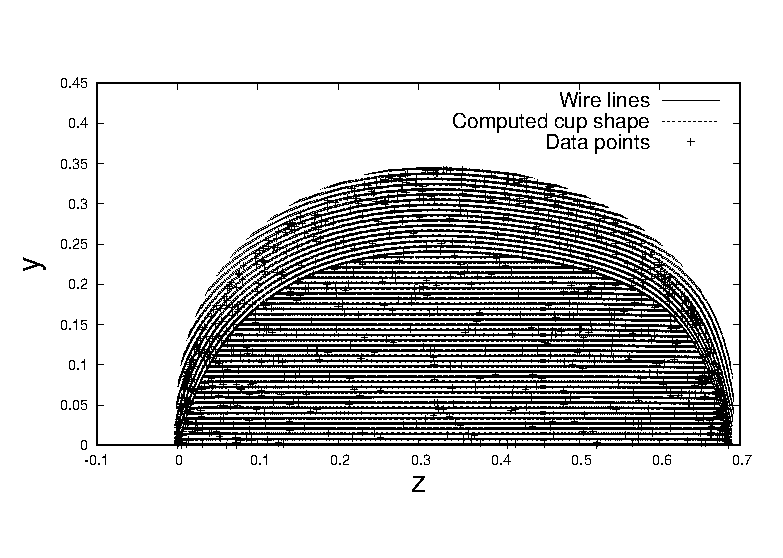
\includegraphics[width=0.6\columnwidth]{./figure/NDS/ObtainedRidgeLinefromz-y.eps}
		\label{fig:zy-NDS}
	}
	\hfil
	\subfigure[xy-view]{
		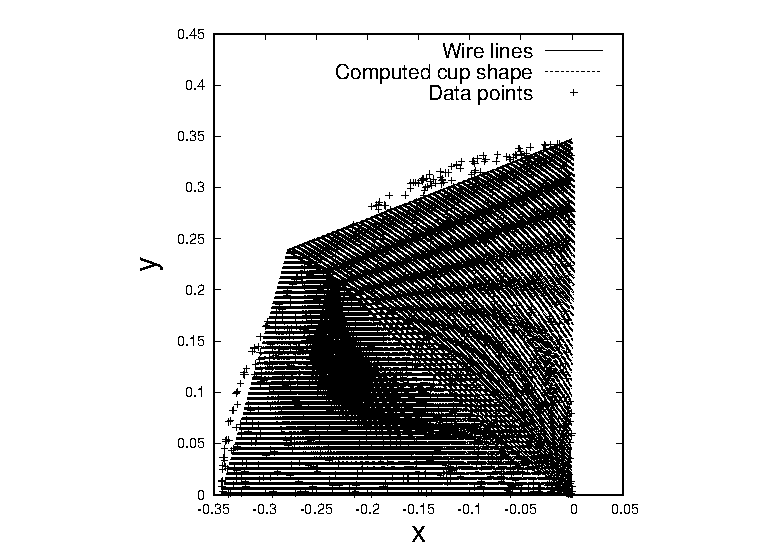
\includegraphics[width=0.6\columnwidth]{./figure/NDS/ObtainedRidgeLinefromx-y.eps}
		\label{fig:xy-NDS}
	}
	\caption{Obtained shape and input data points in Case(1)}
	\label{fig:ObtainedSurfaceNDS}
\end{figure}

\begin{figure}[h!]
	\centering
	\subfigure[LOWER PATTERN]{
		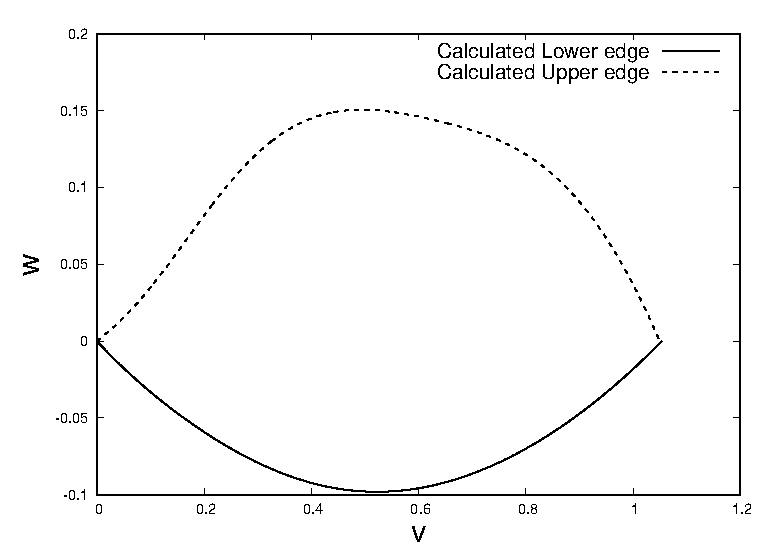
\includegraphics[width=0.6\columnwidth]{./figure/NDS/ObtainedPatternL.eps}
		\label{fig:low-NDS}
	}
	\hfil
	\subfigure[UPPER PATTERN]{
		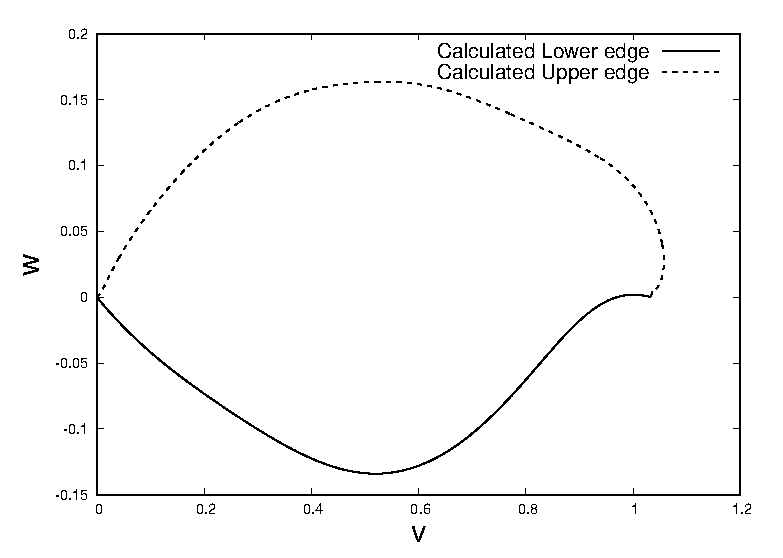
\includegraphics[width=0.6\columnwidth]{./figure/NDS/ObtainedPatternU.eps}
		\label{fig:upp-NDS}
	}
	
	\caption{Obtained patterns in Case(1)}
	\label{fig:ObtainedSurfaceNDS_Pat}
\end{figure}

\begin{figure}[h]
	\centering
	\subfigure[zx-view]{
		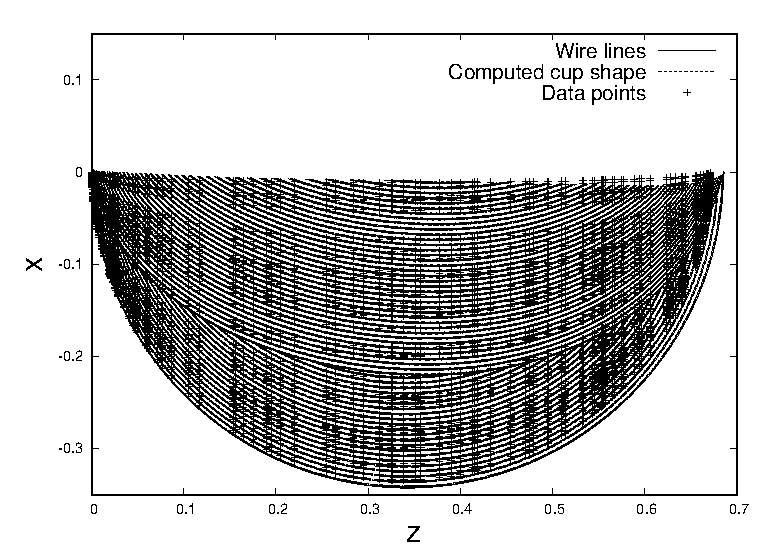
\includegraphics[width=0.6\columnwidth]{./figure/DS/ObtainedRidgeLinefromz-x.eps}
		\label{fig:zx-DS}
	}
	\hfil
	\subfigure[zy-view]{
		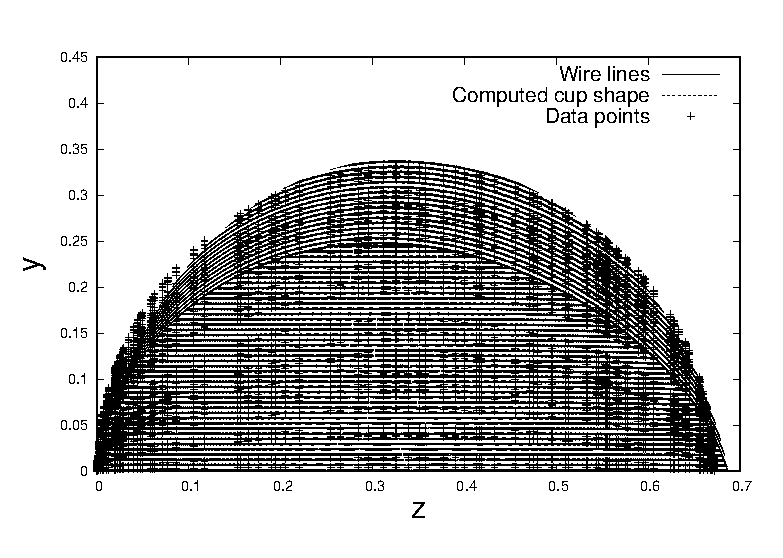
\includegraphics[width=0.6\columnwidth]{./figure/DS/ObtainedRidgeLinefromz-y.eps}
		\label{fig:zy-DS}
	}
	\hfil
	\subfigure[zy-view]{
		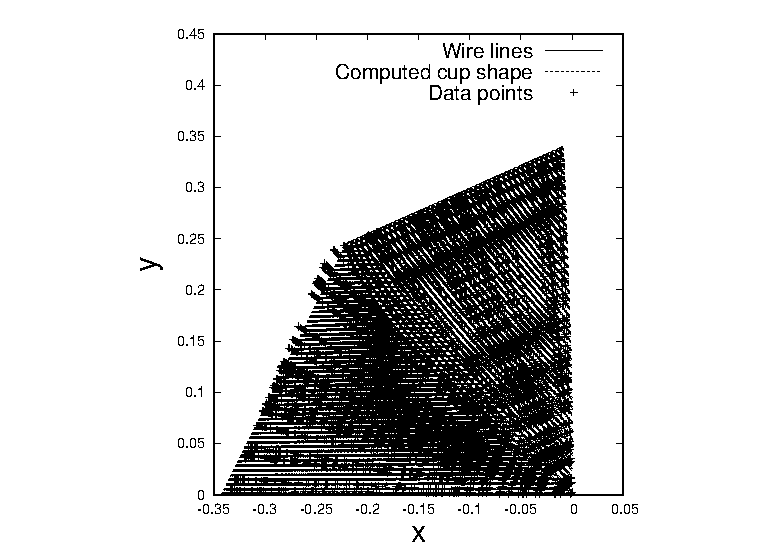
\includegraphics[width=0.6\columnwidth]{./figure/DS/ObtainedRidgeLinefromx-y.eps}
		\label{fig:xy-DS}
	}
	\caption{Obtained shape and input data points in Case(2)}
	\label{fig:ObtainedSurfaceDS}
\end{figure}

\begin{figure}[h!]
	\centering
	\subfigure[LOWER PATTERN]{
		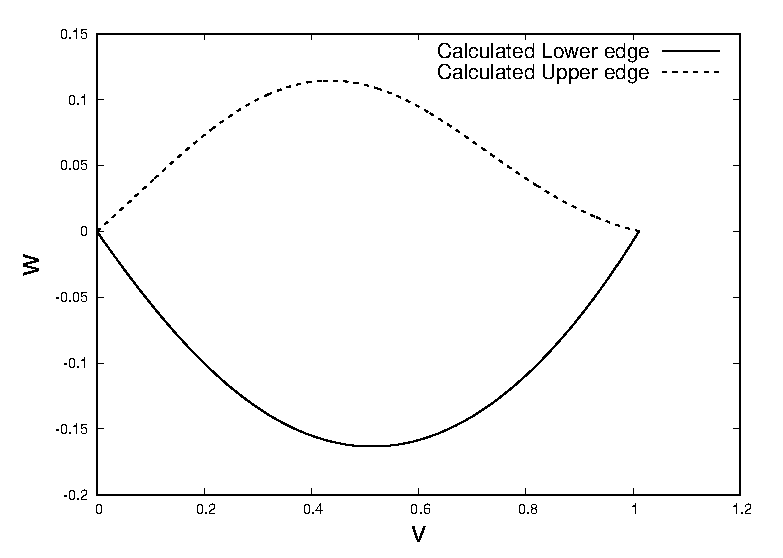
\includegraphics[width=0.6\columnwidth]{./figure/DS/ObtainedPatternL.eps}
		\label{fig:low-DS}
	}
	\hfil
	\subfigure[UPPER PATTERN]{
		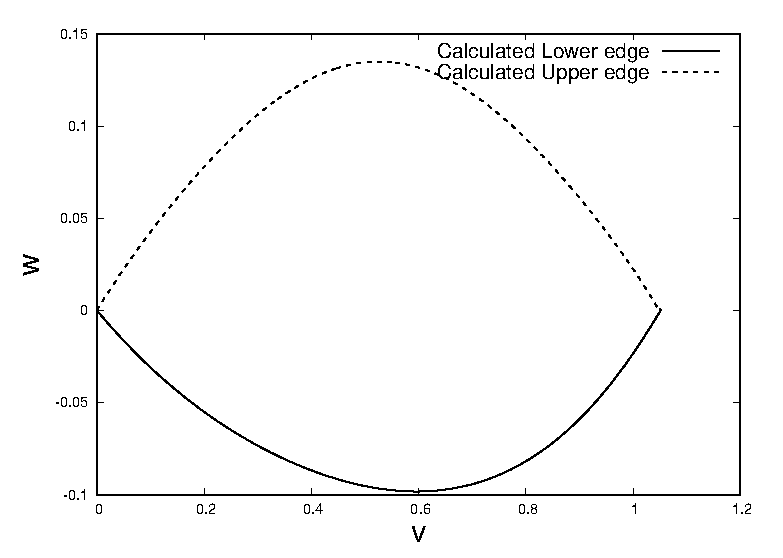
\includegraphics[width=0.6\columnwidth]{./figure/DS/ObtainedPatternU.eps}
		\label{fig:upp-DS}
	}
	
	\caption{Obtained patterns in Case(2)}
	\label{fig:ObtainedSurfaceDS_Pat}
\end{figure}
\section*{CONCLUSION}
In this paper, we proposed a method to design the cup shape of two-piece brassiere cup and its patterns satisfying the function: "fitting to a breast shape", in case that it is given as a cloud of data points. We claimed the background and problem of design process of a brassiere cup. In design process, as a cup model for check of the shapes of patterns is made of paper, it is assumed that the surface of the model is composed of several developable surfaces. At first, we formulated the cup model based on the differential geometry. And we claimed that a developable surface can be determined by two curves included in it. The design process of a two-piece brassiere cup can be converted to the optimization problem, whose objective function is the error between the cup shape and its data points. In order to calculate the error, we first formulated the error between a point and the surface from geometry condition. Then, we proposed a method to divide a data cloud into two clouds: evaluating the lower cup, or evaluating the upper cup. In order to verification of our proposed method, we prepared two examples of data points: a set of non-developable surface and developable surface. From the result of two examples, we confirmed that our proposed method can design the cup shape which manifests the function. As a result, Our proposed method will be useful for efficient design of a two-piece brassiere cup.


%a this paper, a method to design the cup shape of two-piece brassiere cup and its patterns was proposed when its target shape is given as a cloud of data points. As a cup model for check of the shapes of patterns is made of paper, it is assumed that the surface of the model is composed of several developable surfaces. We claimed that a developable surface can be determined by two curves included in it. The design process of a two-piece brassiere cup can be converted to the optimization problem, whose objective function is the error between the cup shape and its data points. In order to calculate the error, we proposed a method to divide a data cloud into two clouds: evaluated by the lower cup, or evaluated by the upper cup. It was experimentally verified that the cup shape calculated by our proposed method reproduced the given data points well. Our proposed method will be useful for efficient design of not only patterns of a brassiere cup but also plate parts of a structure consisting of developable surfaces.

%%%%%%%%%%%%%%%%%%%%%%%%%%%%%%%%%%%%%%%%%%%%%%%%%%%%%%%%%%%%%%%%%%%%%%
%\bibliography{asme2ebackup}

\begin{thebibliography}{99}
	
	\bibitem{c1}Yukiko Higuchi, {\it Sensory test of brassiere}, in The Japanese Journal of Ergonomics, Volume 20, Issue 2, 1984, pp.73-80, (Japanese).
	\bibitem{c2} P.Bo and W.Wang, {\it "Geodesic-Controlled Developable Surfaces for Modeling Paper Bending"}, in Computer Graphics Forum, Volume 26, 2007, pp.365-374.
	\bibitem{c3} H.Pottmann and J.Wallner, {\it "Approximation algorithms for developable surfaces"}, in Computer Aided Geometric Design, Volume 16, 1999, pp.539-556.
	\bibitem{c4} K.Rose, A.Sheffer, J.Wither, M.Cani, and B.Thibert, {\it "Developable surfaces from arbitrary sketched boundaries"}, SGP ’07 Proceedings of the fifth Eurographics symposium on Geometry processing, 2007, pp.163-172.
	\bibitem{c5} G.Aumann, {\it "A simple algorithm for designing developable Bezier surfaces"}, in Computer Aided Geometrix Design Volume 20, 2003, pp.601-619.
	\bibitem{c6} B.Ravani and T.S. Ku, {\it "Bertrand offsets of ruled and developable surfaces"} in Computer-Aided Design Volume 23, 1991, pp.145-152. 
	\bibitem{c7}R.M.C Bodduluri and B.Ravani, {\it "Design of developable surfaces using duality between plane and point geometries"}, in Computer Aided Design Volume 25, 1993, pp.621-632.
	\bibitem{c8}M. Peternell, {\it "Developable surface fitting to point clouds"}, in Computer Aided Design Vol.21, 2004, pp.785-803.
	\bibitem{c9}H.-Y. Chen, I.-K. Lee, S. Leopoldseder, H. Pottmann, T. Randrup , J. Wallner, {\it "On Surface Approximation using Developable Surfaces"}, Graphical Models and Image Processing, Volume 61, Issue2, 1999, pp.110-124
	\bibitem{c10} H.Wakamatsu, Y.Ryu, E.Morinaga, E.Arai, and T. Kubo, M.Oyama, and T.Kishimoto, {\it "3D Shape Prediction of A Paper Model of Two Piece Brassiere Cup for Its Efficient Design"}, Proc.Int. Symp. Flexible Automation, 2016, pp.326-332
	\bibitem{c11} H.Wakamatsu, E.Morinaga, E.Arai, and T. Kubo, {\it "A Virtual Paper Model of a Three Piece Brassiere Cup to Improve the Efficiency of Cup Design Process"}, Proc. 2017 IEEE Int. Conf. on Robotics and Automation, 2017. 
	\bibitem{c12}M.Itoh, and H.Imaoka, {\it "A Method of Prediction Sewn Shapes and a Possibility of Sewing by the Theory of Developable Surfaces"}, J. the Japan Research Association for Textile End-Uses, Volume 48, 2007, pp.42-51, (Japanese).
	\bibitem{MyRef} Kotaro Yoshida, Hidefumi Wakamatsu, Eiji Morinaga, Eiji Arai, Seiichiro Tsutsumi, Takahiro Kubo,{\it "Pattern Shape Optimization of a Two-piece brassiere cup to improve its design efficiency"}, Trans. of the Institute of Systems, Control and Information Engineers, Volume 32, No. 5, 2019, pp. 192-202.
	\bibitem{c13}Elsgolc L.E {\it Calculus of Variations}, Pergamon Press, 1961, pp. 144-157.
\end{thebibliography}

\authorbiography{Kotaro, YOSHIDA}{}{Non-Member}{%
	Kotaro Yoshida received his B.Eng. and M.Eng. degree from Osaka University in 2017 and 2019, respectively. He is doing a doctoral degree at Osaka University.
}

\authorbiography{Hidefumi, ,WAKAMATSU}{}{Member}{%
	HidefumiWakamatsu received his B.Eng.,
	M.Eng. and Ph.D. degrees from Osaka
	University, Japan, in 1993, 1994 and
	2001, respectively. From 1995 to 2006,
	he worked as a Research Associate, Osaka
	University. He then became an Associate
	Professor at Division of Materials and Manufacturing
	Science, Osaka University. His research interests
	include handling of flexible object. He is a member of
	RSJ, JSME, JSPE, JWS and TMSJ.
}

\authorbiography{Eiji, ,MORINAGA}{}{Member}{%
	Eiji Morinaga received his B.Eng., M.Eng.
	and Ph.D. degrees in Mechanical Engineering
	from Osaka University, Japan,
	in 2000, 2002 and 2005, respectively. From
	2005 to 2007, he worked as a Designated
	Researcher at Center for Advanced Science
	and Innovation, Osaka University. He then became
	an Assistant Professor at Division of Materials and Manufacturing
	Science, Osaka University. His research interests
	include system design and integration in product design
	and manufacturing. He is a member of JSME, JSPE,
	JWS, JIEP and TMSJ.
}

\authorbiography{Takahiro, ,KUBO}{}{Non-Member}{%
	Takahiro Kubo received his B.A. degree in Sport Sciences from Waseda University, Japan, in 2007, and M.A. degree in Arts and Sciences from Tokyo University, Japan, in 2010. He then joined Wacoal Corp. His position is in Human Science Research Center.
}


\end{document}
%
%% end of paper.tex
